\section{Introduction}

Emulsions formed from mixtures of immiscible liquids are widely used as structural 
templates for fabricating porous materials. These include a broad array of applications 
such as porous polymers, ceramics, synthetic nanoparticles, and engineered tissue scaffolds 
\cite{zhang_emulsion_2019, stubenrauch_emulsion_2018, jones_high-temperature_2009, binks_macroporous_2002, aldemir_dikici_basic_2020}. 
The technique of emulsion templating 
provides a flexible and efficient approach to controlling key structural features of the final
material—namely, the domain size, volume fraction, and phase composition—by manipulating the 
formulation and processing conditions of the emulsion \cite{mudassir_fundamentals_2021}. To ensure 
thermodynamic and mechanical stability during processing, emulsions are typically stabilized by additives. 
Among these, particle-stabilized systems—commonly referred to as Pickering emulsions—have emerged as attractive 
alternatives to traditional surfactant-based emulsions due to their ability to form stable interfaces without 
relying on potentially harmful chemicals \cite{ramsden_separation_1904, zheng_pickering_2022, menner_particle-stabilized_2007}.

A particularly intriguing subclass of Pickering emulsions is the bicontinuous interfacially jammed emulsion gel, or bijel. 
Bijels are characterized by a tortuous co-continuous morphology where two fluid phases are separated by a particle-laden 
interface \cite{cates_bijels_2008}. This structure forms when a binary liquid mixture containing colloidal particles is 
rapidly quenched into a spinodal decomposition regime. As phase separation proceeds, the particles are swept up by the 
growing interface. Eventually, particle crowding leads to jamming at the interface, effectively halting further coarsening 
and locking the structure into a bicontinuous state. Bijels were first observed in simulation studies \cite{stratford_colloidal_2005}, 
and later successfully fabricated in experimental systems involving water-lutidine mixtures stabilized with silica particles 
\cite{clegg_emulsification_2007, herzig_bicontinuous_2007}. Since these foundational discoveries, a wide range of bijel 
formulations and processing techniques have been developed to enable greater scalability and control. Notably, 
Haase et al.~\cite{haase_continuous_2015} introduced solvent transfer-induced phase separation (STRIPS), a scalable 
and continuous fabrication method that leverages imposed flow fields to direct droplet and jet formation. As a result 
of these innovations, bijels have gained widespread interest as structural templates for functional materials, including 
filtration membranes, electrochemical electrodes, and biocompatible scaffolds 
\cite{yabuno_preparation_2020, pang_highly_2020, witt_microstructural_2016, thorson_composite_2018}.

Beyond chemical composition, the geometry of the stabilizing particles plays a critical role in determining 
the microstructure and stability of emulsions. When anisotropic particles—such as ellipsoids or rods—adsorb at 
fluid interfaces, they give rise to shape-dependent capillary interactions that are markedly different from those 
induced by spherical particles \cite{loudet_capillary_2005,madivala_exploiting_2009}. These interactions can 
significantly enhance emulsion stability, as demonstrated by Madivala et al., and often result in distinct particle 
arrangements at the interface \cite{madivala_self-assembly_2009}. Moreover, anisotropic particles are capable of 
self-assembling in response to interface curvature gradients, where the curvature acts as an external field influencing 
particle orientation and spatial distribution \cite{cavallaro_curvature-driven_2011, furst_directing_2011}. Computational 
studies, including Monte Carlo and Lattice Boltzmann simulations, have provided insight into how such particles dynamically 
interact with fluid interfaces \cite{bresme_orientational_2007, bresme_computer_2008, gunther_lattice_2013,gunther_timescales_2014}. 
These simulations show that anisotropic particles introduce additional timescales during 
emulsion formation due to their rotational behavior. Initially, they rotate to align their major axes with the interface, 
and later reorient under capillary forces, contributing to prolonged coarsening and finer domain features. Experimental studies 
by Hijnen et al.~\cite{hijnen_bijels_2015} confirmed that rod-shaped particles can jam more quickly than spheres at smaller 
interfacial separations and can even tilt out of the plane due to compression during domain evolution.

Incorporating magnetic functionality into particle stabilizers introduces the possibility of externally controlling interfacial 
behavior using applied magnetic fields \cite{melle_pickering_2005, zhou_magnetic_2011}. Magnetic particles can align or assemble 
in response to external fields, enabling modulation of both emulsion stability and particle organization at the interface 
\cite{dassanayake_structure_2000, leunissen_directing_2009}. This is especially pronounced in systems containing anisotropic magnetic 
particles, where external fields can trigger orientation transitions and alter capillary interactions 
\cite{morgan_understanding_2013, davies_interface_2014, davies_dipolar_2015}. However, not all particle geometries respond equally. 
Simulations by Kim et al. revealed 
that magnetic fields exert minimal influence on the microstructure of bijels stabilized by spherical particles \cite{kim_bijels_2010}. 
In contrast, Carmack and Millett demonstrated that applying electric fields to bijels stabilized with dielectric particles can induce 
significant morphological changes, including domain alignment and cylindrical channel formation via field-induced dipolar interactions 
\cite{carmack_tuning_2018}. These results suggest that the interplay between field direction, particle geometry, and interface dynamics 
can be exploited to engineer emulsion microstructures in situ.

This chapter investigates how external magnetic fields influence the formation and microstructure of bijels stabilized by anisotropic 
magnetic particles. Using a hybrid simulation framework combining Lattice Boltzmann and Molecular Dynamics, we model the phase separation 
of binary fluids containing anisotropic particles with permanent dipole moments aligned along their symmetry axes. By systematically varying 
magnetic flux density and particle aspect ratio, we assess how these parameters affect domain structure, spacing, and tortuosity. Our 
findings reveal that, while magnetic fields do not inhibit bijel formation, they significantly impact the resulting morphology. 
Specifically, anisotropic particles subjected to magnetic torque align during formation, leading to anisotropic domain features and 
enhanced interfacial order. This reorientation improves packing efficiency and delays the onset of interfacial jamming. Compared to 
field-free cases, the resulting bijels display a higher degree of structural organization. These results underscore the potential of 
magnetic anisotropic particles as tools for designing responsive, field-tunable porous materials.

\section{Results}

The transport characteristics of Bijels are closely linked to the morphology of the underlying 
phase-separated bijel template. In this study, we investigate how domain size and tortuosity evolve in bijels stabilized by anisotropic particles, 
with a particular focus on the influence of magnetic fields during formation.
To this end, we simulate bijels composed of ellipsoidal magnetic particles at a fixed particle volume fraction of \(\phi_p = 0.15\), systematically 
varying the applied magnetic flux density such that the Bond number spans the range \(0 \le \bar{B} \le 1\). Our approach isolates the effects of 
the magnetic field on microstructure while holding other parameters constant. Prior studies have explored how changes in particle concentration and 
interfacial tension affect bijel morphology—for example, work by Hijnen et al.~\cite{hijnen_bijels_2015} and Jansen and Harting~\cite{jansen_bijels_2011}.

\begin{figure}
    \centering
    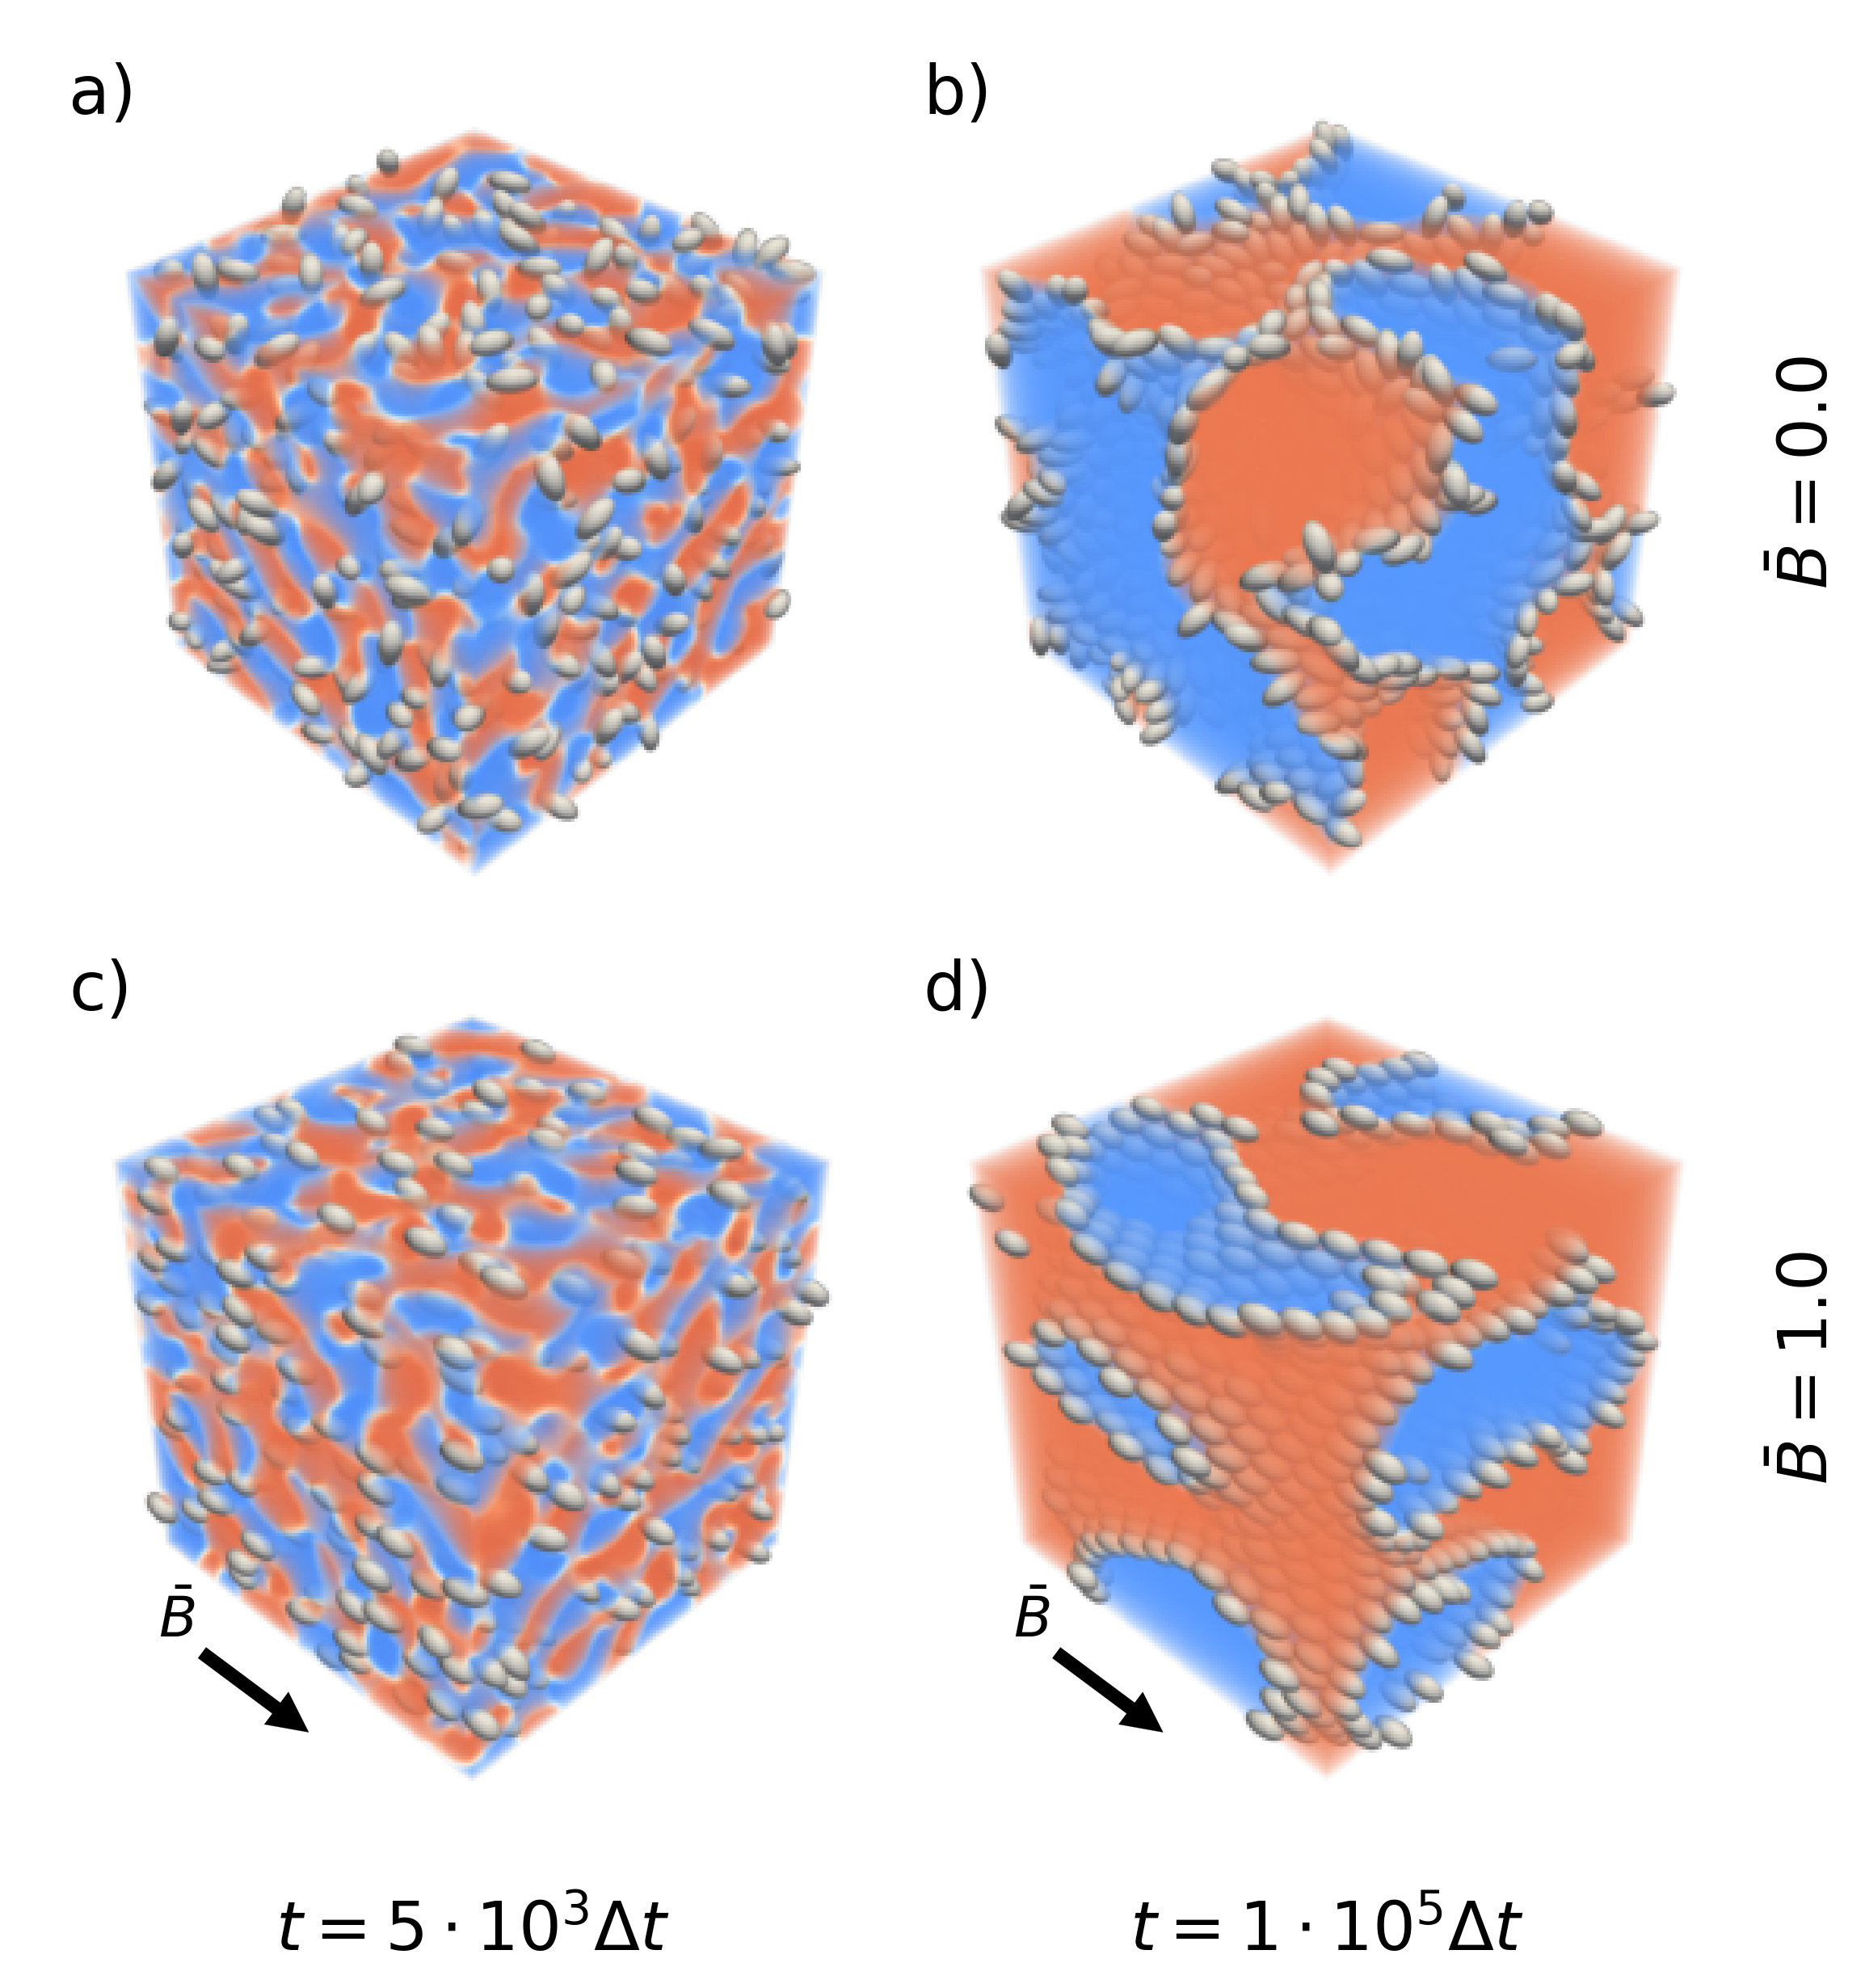
\includegraphics[scale=0.6]{../figures/results/paper1/microstructure_viz.png}
    \caption{Snapshots of emulsion gels stabilized by prolate ellipsoids after $t=5\cdot10^3$ timesteps (left) and after $10^5$ timesteps (right). 
             The top row shows the structure forming without a magnetic field. The bottom row shows the structure forming in an applied magnetic 
             field of reduced strength $\bar{B}=1.0$. The snapshots are colored according to the order parameter $\phi$.}
    \label{fig:microstructure_viz}
\end{figure}

Figure~\ref{fig:microstructure_viz} presents snapshots of bijel structures at various time points, comparing systems formed with and without an applied 
magnetic field. These images demonstrate how anisotropic particles align along the field direction, causing interfacial deformation and rearrangements 
such as domain reorientation, coalescence, or breakup. This alignment appears to result in larger characteristic domain sizes when magnetic fields are 
applied. A detailed, quantitative analysis of the impact of magnetic fields on bijel morphology—particularly domain size—is presented in the following sections.
    
\subsection{Structure factor and domain size of magnetically responsive bijels}
    
    In LB simulations of spinodal decomposition
    \cite{kendon_3d_1999,kendon_inertial_2001}, a characteristic length
    scale can be obtained from the structure factor
    %
    \begin{equation}
    S(\vec{k},t) = \tilde{\phi}(\vec{k},t)\tilde{\phi}(-\vec{k},t) .
    \end{equation}
    %
    where \(\tilde{\phi}(\vec{k},t)\) is the Fourier
    transform of the order parameter fluctuations
    \(\phi(\vec{x},t)-\left\langle\phi\right\rangle\). A common measure of
    domain size uses the spherically averaged structure factor
    %
    \begin{equation}
    S(k,t) = \frac{1}{n_k} \sum_{k-\frac{\Delta}{2}<k<k+\frac{\Delta}{2}} \tilde{\phi}(\vec{k},t)\tilde{\phi}(-\vec{k},t) ,
    \end{equation}
    %
    where \(k=|\vec{k}|\) denotes the modulus of \(\vec{k}\)
    and \(n_k\) is the number of lattice sites in a shell of radius \(k\)
    and thickness \(\Delta=2\pi/L_V\). The average domain size can then be
    defined in terms of the \(n\)-th moment of the structure factor
    \cite{laradji_molecular_1996}
    %
    \begin{equation}
        L_n(t) = 2\pi \left( \frac{\sum_k S(k,t)}{\sum_k k^n S(k,t)} \right)^{\frac{1}{n}}
    \end{equation}
    
The average domain size defined here may not directly match the visually estimated size seen in snapshots such as Fig.~\ref{fig:microstructure_viz}. 
However, in the dynamic scaling regime, different domain size metrics typically differ only by a constant factor. We observed that the commonly used 
measure \(L_1(t)\) tends to overestimate the apparent domain size. This is partly due to poor statistics in the low-\(k\) shells of the spherically 
averaged structure factor, where the average \(|\vec{k}|\) deviates from the nominal shell radius. Additionally, simulations with periodic boundaries 
are subject to finite-size effects. In systems with anisotropic particles, the structure factor is generally not isotropic. To account for this, we 
also computed directional domain sizes along each Cartesian axis from the 3D structure factor using second-moment analysis \cite{jansen_bijels_2011, 
gunther_timescales_2014}.

    %
    \begin{equation}
    L_\beta(t)=2\pi\sqrt{\frac{\sum_{\vec{k}}S(\vec{k},t)}{\sum_{\vec{k}}k_\beta^2 S(\vec{k},t)}} .
    \end{equation}
    %
    This allows us to compute a domain size parallel
    (\(L_\parallel=L_z\)) and perpendicular (\(L_\perp=(L_x+L_y)/2\)) to the
    direction of \(\vec{B}\) separately. The average domain size \(L_d(t)\)
    is computed as \(L_d(t)=\sum_\beta L_\beta(t) / 3\).
    %
    \begin{equation}
    L_d(t)=2\pi\sqrt{\frac{\sum_{\vec{k}}S(\vec{k},t)}{\sum_{\vec{k}}\sum_\beta k_\beta^2 S(\vec{k},t)}} .
    \end{equation}
    %
    
Before computing the structure factor \(S(\vec{k}, t)\), we filled lattice sites occupied by particles with the average density of 
their neighboring fluid nodes. This was done using an iterative method that applies Eq.~\eqref{eq:fill_particles}, starting from the 
particle surface and proceeding layer by layer until all solid nodes were filled. The order parameter \(\phi(\vec{x}, t)\) was then 
computed from the resulting filled density fields \(\rho_k(\vec{x}, t)\). This filling procedure is essential to eliminate spurious 
oscillations in the structure factor at length scales comparable to the particle size.
    
    
    \begin{figure*}
        \centering
        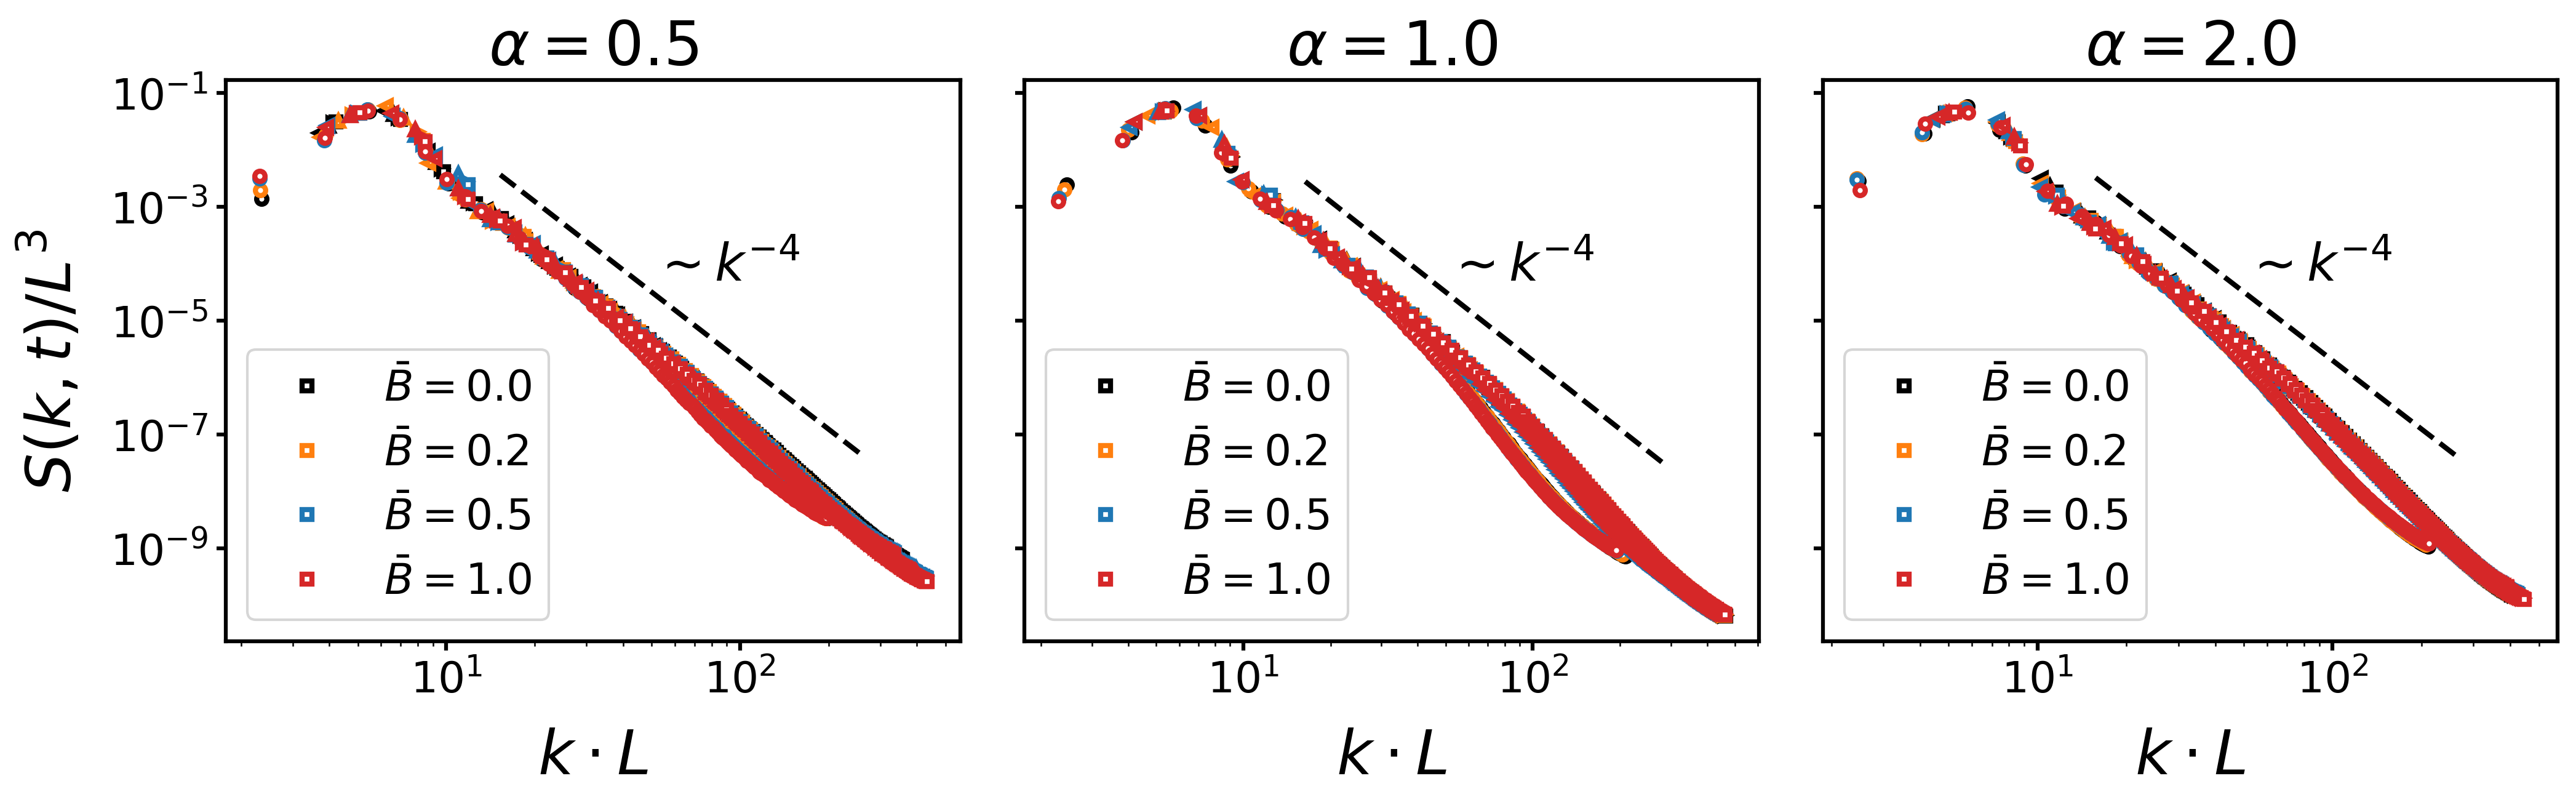
\includegraphics[width=\textwidth]{../figures/results/paper1/structure_factor.png}
        \caption{Scaling plot of the dynamic structure factor $S(k,t)$ for different particle shapes $\alpha$ and at different magnetic field 
                 strength $\bar{B}$. The structure factor is plotted at four different timesteps for each case. The good data collapse shows 
                 that the bijel formation is driven by spinodal decomposition. The decay to the right of the peak is reasonably well described 
                 by Porod's law $S(k)\sim k^{-4}$.}
    \label{fig:structure_factor}
    \end{figure*}
    
Figure~\ref{fig:structure_factor} shows the scaling behavior of the dynamic structure factor \(S(k, t)\). While the data exhibit good overall 
collapse, deviations from dynamic scaling appear at smaller length scales. The post-peak decay follows Porod's law, \(S(k) \sim k^{-4}\), indicating 
scattering from relatively flat interfaces. These findings are consistent with results by Kendon et al.~\cite{kendon_3d_1999, kendon_inertial_2001} 
for spinodal decomposition in binary fluids, supporting the view that bijel formation is initially governed by fluid demixing dynamics. Particle effects 
become significant only at later stages, when interface coarsening reduces available surface area and triggers particle interactions. This leads to jamming, 
which is reflected in the abrupt slowing of domain growth, as shown in Figure~\ref{fig:domain_size}.


\begin{figure*}
    \centering
    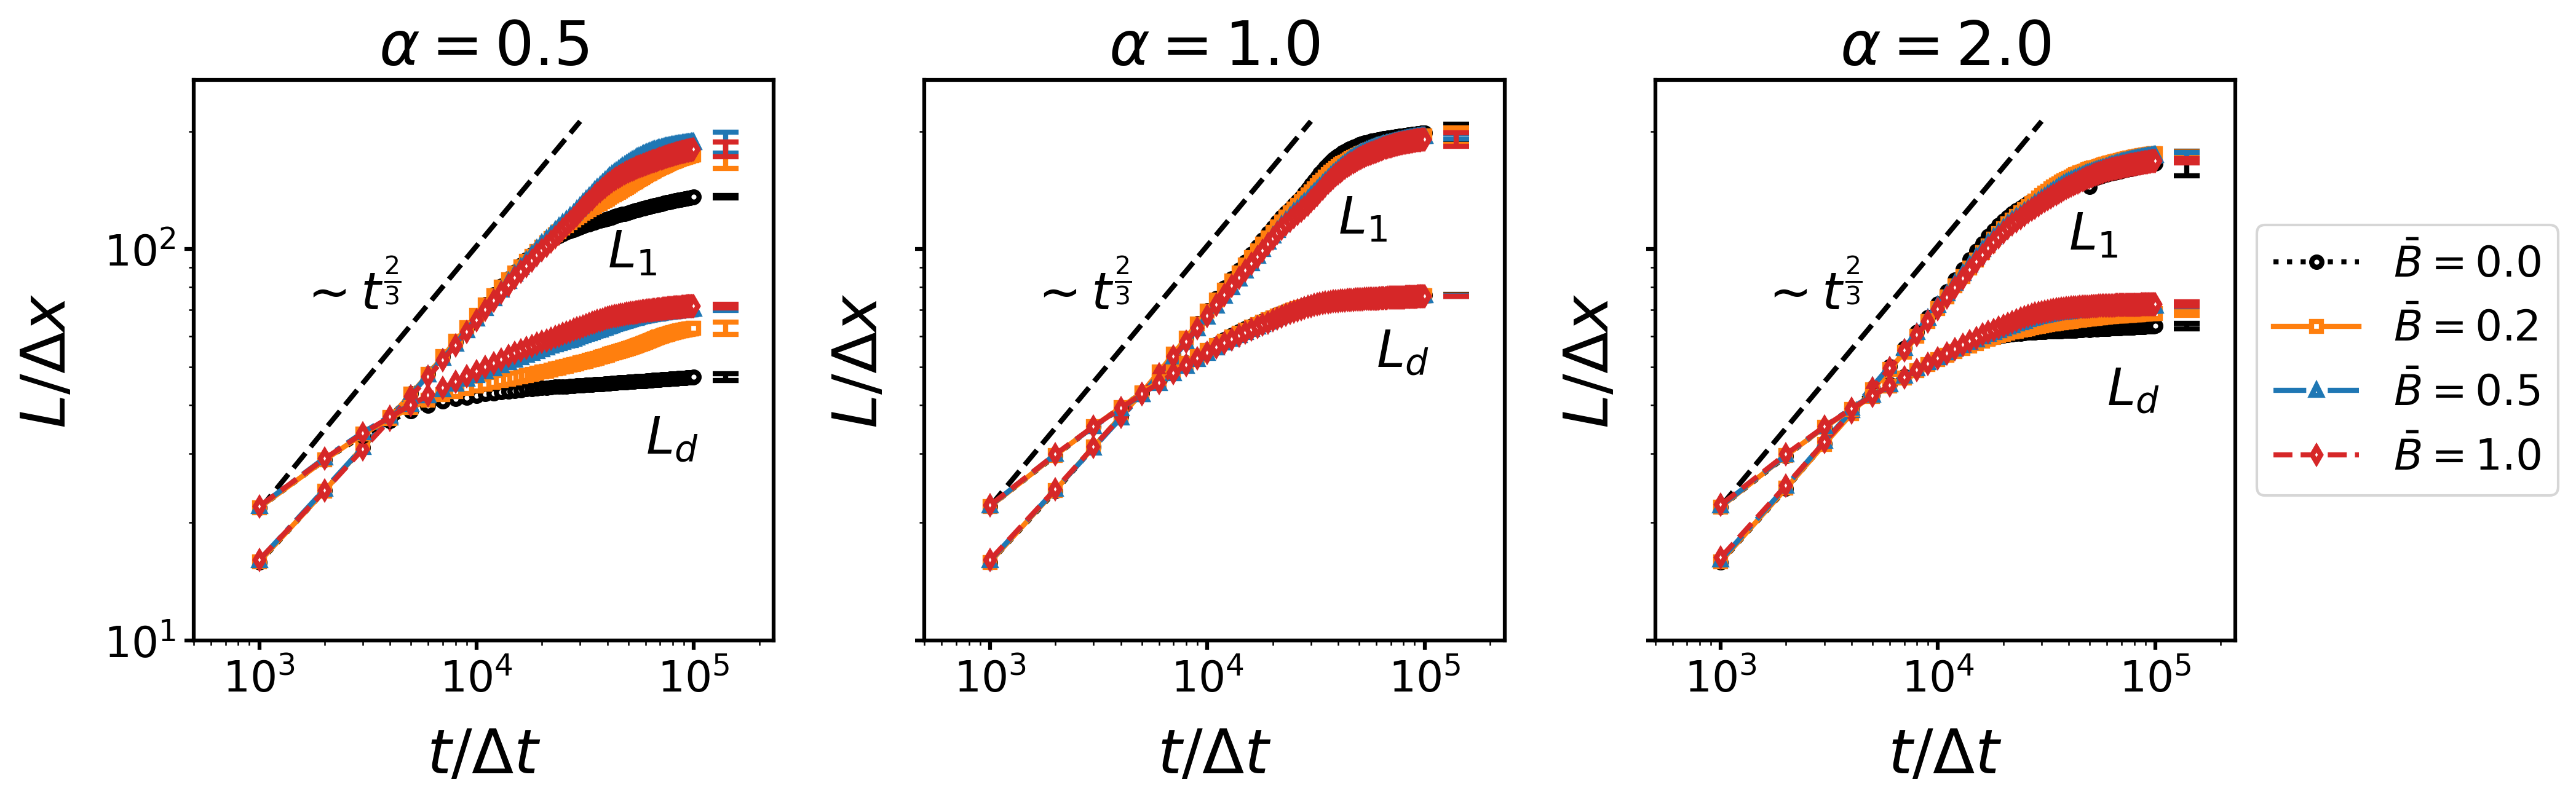
\includegraphics[width=\textwidth]{../figures/results/paper1/domain_size.png}
    \caption{Time dependence of the average domain size of the bijel for different particles shapes $\alpha$ and at different magnetic field strength $\bar{B}$. $L_1$ denotes the domain size obtained from the first moment of the spherical average structure factor, and $L_d$ denotes the domain size obtained from the second moment of the 3D structure factor. The increase roughly follows a $\sim t^{2/3}$ scaling law indicative of the inertial regime of spinodal decomposition.}
    \label{fig:domain_size}
\end{figure*}
    
A nonlinear fit of the domain size with form \(b(t - t_0)^a\) over the time interval \(t \in [0,\ 3 \cdot 10^5 \Delta x]\) yields scaling exponents of \(a = 0.6448\) 
for spherical particles, \(a = 0.6083\) for oblate particles with aspect ratio \(\alpha = 0.5\), and \(a = 0.652\) for prolate ellipsoids with \(\alpha = 2\). 
These values are consistent with the theoretical exponent \(a = 2/3\), characteristic of the inertial scaling regime, where the characteristic velocity 
\(U = dL/dt\) scales as \(U \sim \sqrt{\sigma / (\rho L)}\), resulting in \(L \sim t^{2/3}\).
Beyond approximately 30,000–40,000 time steps, domain growth slows down and approaches a steady-state value. The plateau values are \(L_1 \approx 200 \Delta x\) 
for spherical particles, \(L_1 \approx 180 \Delta x\) for prolate particles, and \(L_1 \approx 170 \Delta x\) for oblate particles.
    
In contrast, an alternative measure of domain size, \(L_d\), obtained from the second moments of the full 3D structure factor, does not exhibit the same 
power-law growth. Its increase is significantly slower, with fitted exponents ranging from 0.12 to 0.20. Moreover, \(L_d\) saturates earlier and reaches a 
plateau near \(L_d \approx 70 \Delta x\) for all particle shapes. Although dynamic scaling permits different length scale measures to vary by a constant 
factor, the deviation of \(L_d\) from both viscous and inertial scaling suggests that it may not serve as a reliable characteristic length scale.
    
Interpreting the structure factor moments as statistical moments of a probability distribution, the second moment of the 3D structure factor corresponds to 
the ratio of the fourth and second moments of the spherically averaged structure factor—due to the \(k^2\) weighting in the volume integral. Thus, \(L_d\) 
may be more appropriately viewed as a descriptor of the structure factor's shape (akin to kurtosis), rather than as a direct measure of domain size.
Nonetheless, the directional second moments \(L_\beta\) provide independent domain size estimates along each Cartesian axis, making them valuable for 
identifying anisotropy in the domain morphology.
    
    
\subsection{Effect of magnetic field on bijel formation}
    
    \begin{figure}
    \centering
    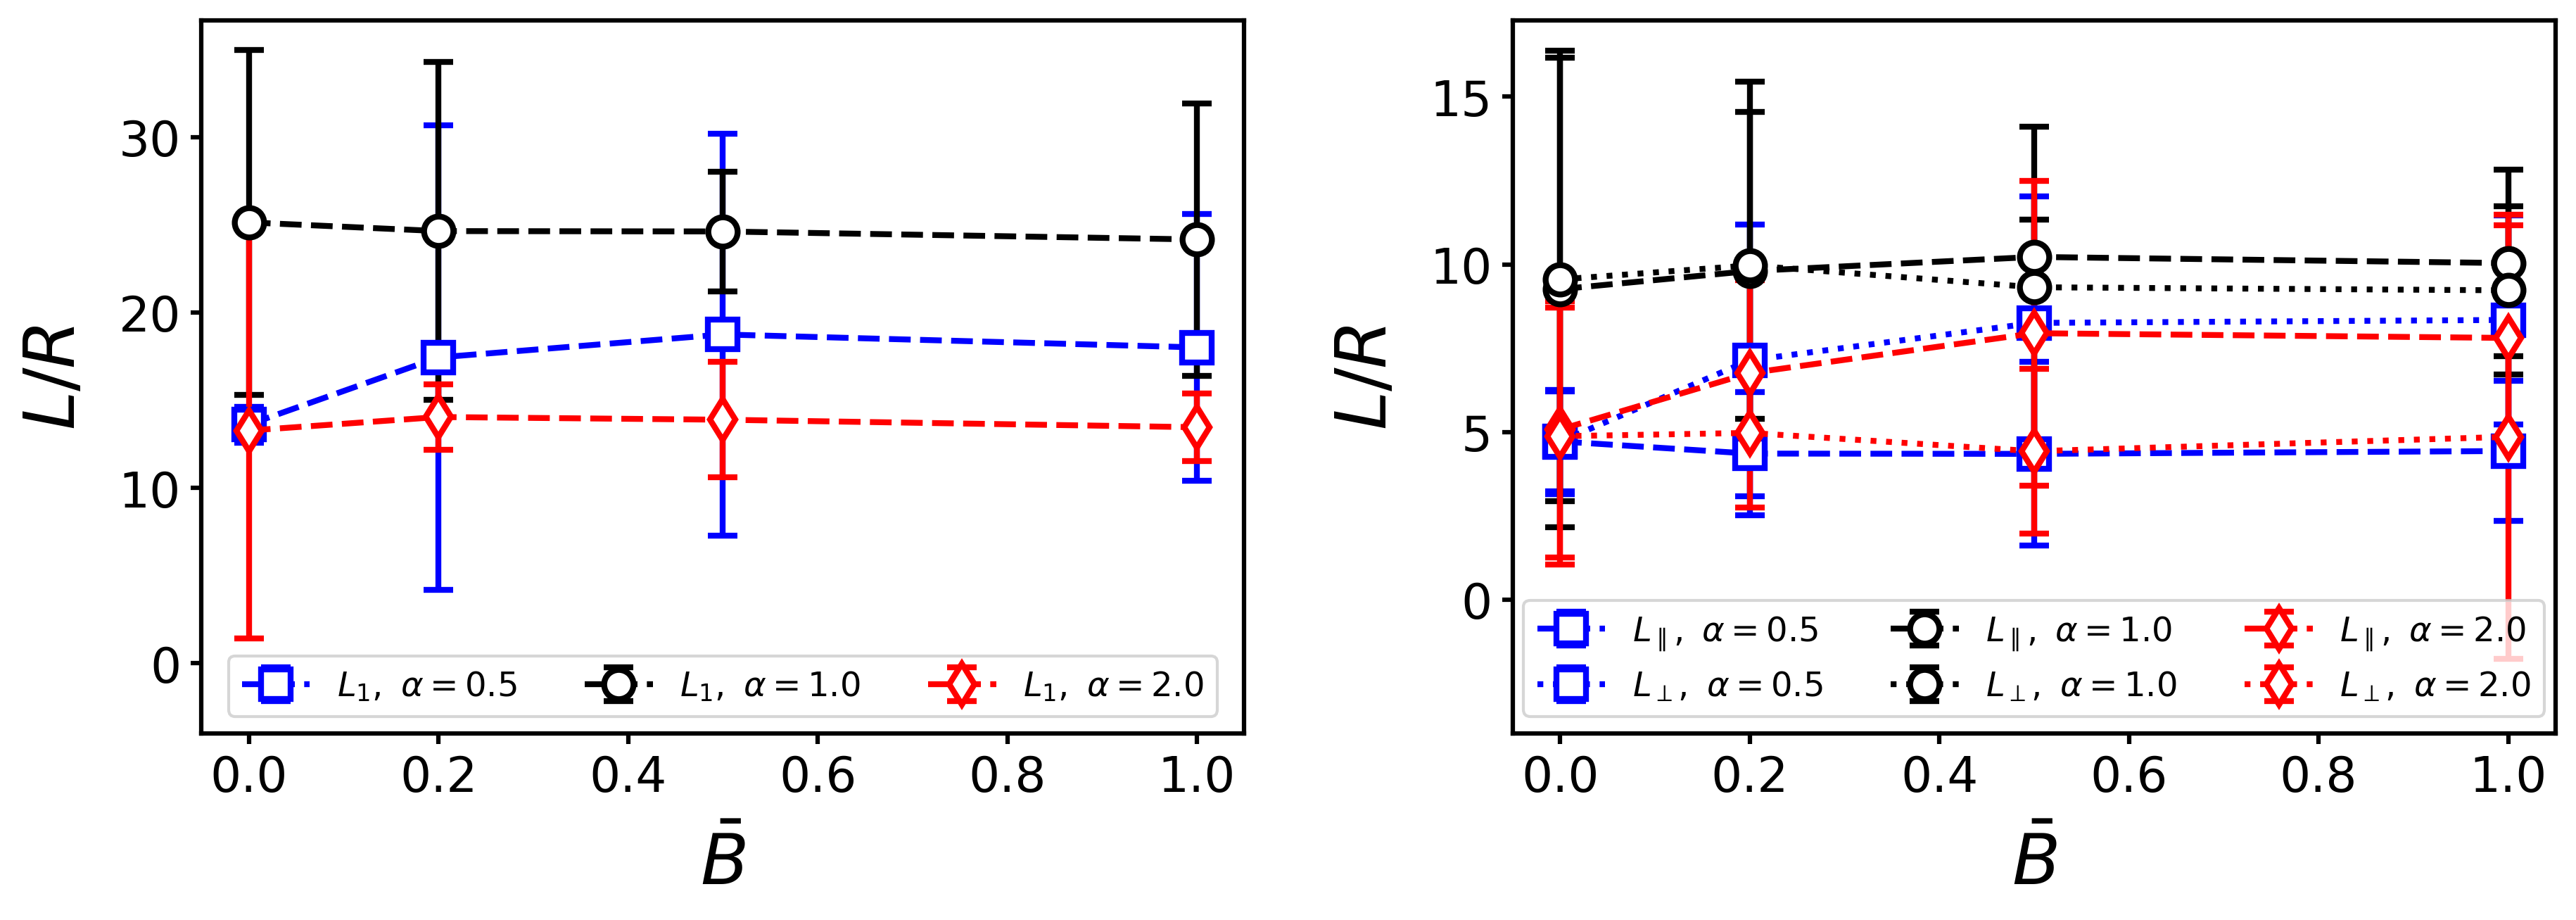
\includegraphics[width=\columnwidth]{../figures/results/paper1/D2a-vs-B_ss.png}
    \caption{Dependence of the average domain size on the magnetic field strength $\bar{B}$. The left plot shows the average domain size $L_1$ obtained from the spherically averaged structure factor. The right plot shows the parallel and perpendicular domain size obtained from the respective second moments of the 3D structure factor. Errorbars indicate the standard deviation taken over three independent simulation runs. For anisotropic particles, the directional domain size becomes more anisotropic with increasing field strength.}
    \label{fig:D2a_B}
    \end{figure}

To understand the microstructure changes imparted onto the bijel, we plot the domain size \(L_d\) at the final timestep in 
Figure~\ref{fig:D2a_B}a, normalized by \(R\), the larger semi-axis of the ellipsoidal particles. Each point 
represents the final domain size, averaged over three simulations with identical parameters. This normalization highlights that ellipsoidal particles 
reduce the domain size in bijels, consistent with findings by Günther et al.~\cite{gunther_timescales_2014}. Ellipsoids stabilize a larger interfacial 
area relative to their volume due to their greater cross-sectional area. Additionally, steric effects limit how densely anisotropic particles can pack, 
a topic we discuss further below.

Figure~\ref{fig:D2a_B}b displays the domain size components parallel and perpendicular to the applied magnetic field \(\vec{B}\). For prolate particles, 
the domain size increases by up to three particle radii at the highest field while the perpendicular size remains unchanged. The 
trend reverses for oblate particles, where the parallel domain size slightly decreases and the perpendicular size increases by about four particle radii.
Without a magnetic field, prolate particles yield smaller domains than spherical or oblate ones. However, under field influence, they increase domain size. 
This anisotropy results from particle alignment under the magnetic field. The difference between prolate and oblate behavior 
stems from the dipole orientation. \(\vec{m}\) aligns with the major axis in prolates (within the larger cross-section plane) and the minor axis in oblates 
(perpendicular to it). Thus, field-induced alignment encourages tighter packing perpendicular to \(\vec{B}\) for prolates and parallel for oblates. These 
effects saturate at intermediate field strengths, with little change at higher values.

    
\subsection{Tortuosity}
    
    \begin{figure*}
    \centering
    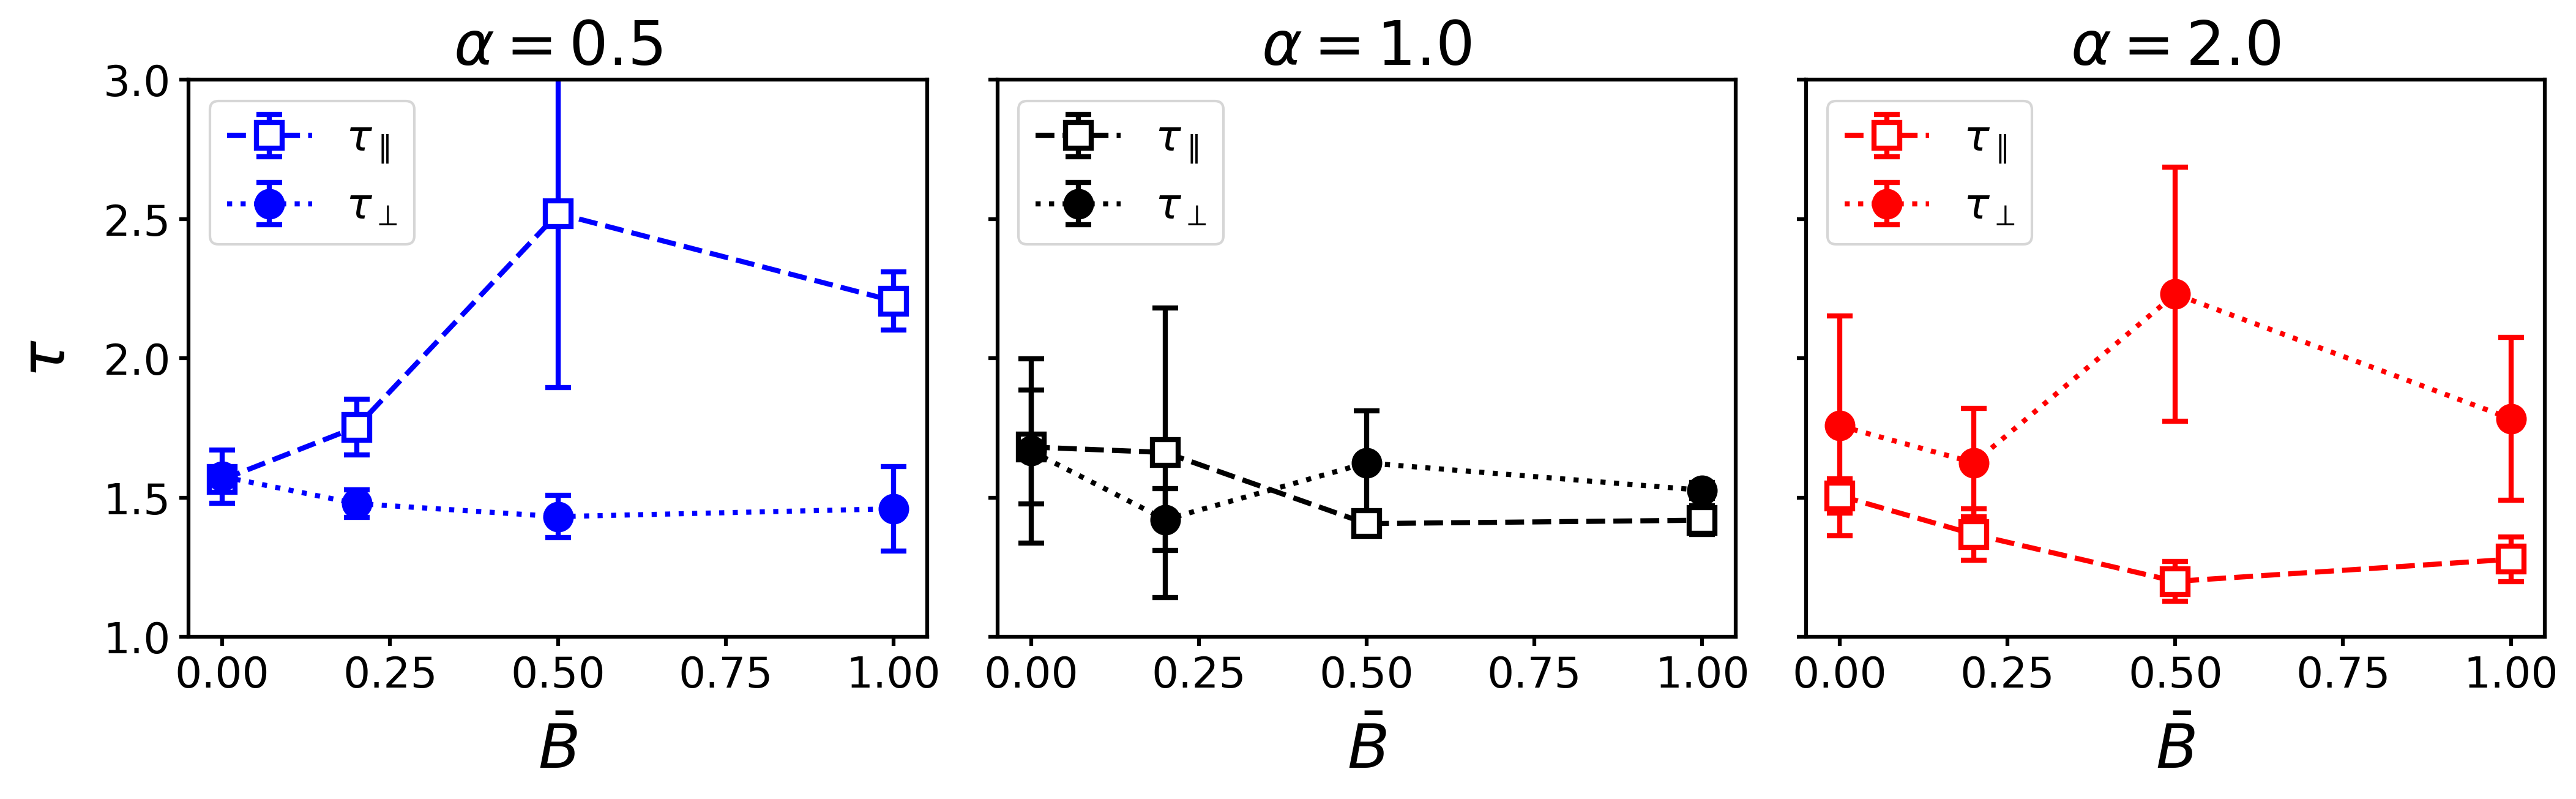
\includegraphics[width=\textwidth]{../figures/results/paper1/tortuosity_compare.png}
    \caption{Dependence of the tortuosity on the magnetic field strength $\bar{B}$ for different particle shapes $\alpha$. Different components of the tortuosity tensor show the anisotropy for oblate and prolate particles.}
    \label{fig:tau_B}
    \end{figure*}

The observed anisotropy in domain size suggests that magnetic fields influence bijel morphology at the microscale. To determine whether these structural 
changes impact macroscopic transport properties, we also analyzed the tortuosity of the bijels. While geometric, 
diffusional, and hydraulic definitions of the tortuosity exist, we use the diffusional tortuosity, defined as \(\tau = \epsilon D / D_{\text{eff}}\), 
where \(D_{\text{eff}}\) is the effective diffusivity and \(D\) is the intrinsic molecular diffusivity. \cite{dasilva_tortuosity_2022} Porous structures were 
extracted by binarizing the final order parameter field using a zero threshold, isolating the largest connected (percolating) domain. We computed tortuosity 
along each Cartesian direction using the \texttt{taufactor} package \cite{cooper_taufactor_2016}, which compares steady-state diffusion through the porous 
structure to bulk diffusion in an equivalent volume. Periodic boundary conditions were applied via the \texttt{PeriodicSolver}.

Figure~\ref{fig:tau_B} presents tortuosity as a function of magnetic flux density for the three particle aspect ratios. In the absence of a field, all 
shapes yield a similar tortuosity around \(\tau \approx 1.5\), slightly exceeding the Bruggeman prediction \(\tau = \epsilon^{-0.5} = 1.41\) for equal 
phase volume fractions \(\epsilon = 0.5\) \cite{bruggeman_berechnung_1935, tjaden_origin_2016}. These values align with simulations of gyroid structures 
by Luo et al., who reported tortuosities between 1.48 and 1.73 \cite{luo_macroscopic_2020}.

Under an applied magnetic field, tortuosity becomes directionally dependent for bijels stabilized by anisotropic particles (\(\alpha \neq 1\)). For oblate 
particles (\(\alpha = 0.5\)), tortuosity increases in the field-parallel direction, while remaining near \(\tau \approx 1.5\) perpendicular to the field. 
In contrast, prolate particles (\(\alpha = 2\)) exhibit the opposite trend: tortuosity rises in the perpendicular direction and slightly decreases along 
the field. These trends align with the anisotropic domain sizes and particle alignment under the field. For prolates, alignment of the major axis with the 
magnetic moment results in larger domains and reduced tortuosity along the field direction.

Notably, the most pronounced tortuosity changes occur at intermediate field strength (\(\bar{B} = 0.5\)), suggesting a nonlinear interplay between magnetic 
and interfacial forces. This highlights that field-induced morphological evolution is more complex than a simple monotonic response, prompting a deeper 
investigation into the bijels microstructural changes.
    
\subsection{Kinetics of bijel formation in magnetic fields}

To better understand the mechanisms driving coarsening, we now examine the kinetics of bijel formation in greater detail. Coarsening behavior 
is quantified through a coarsening velocity, which we compute by taking finite differences of the directional domain size to obtain its individual components
    %
    \begin{equation}
    u_{L_\beta}(t) = \frac{L_\beta(t+\Delta t_s)-L_\beta(t-\Delta t_s)}{2\Delta t_s} ,
    \end{equation}
    %
    where \(\Delta t_s\) is the time between simulation
    snapshots, and $\beta$ denotes either the direction parallel or perpendicular to the magnetic field.
    
    \begin{figure*}
    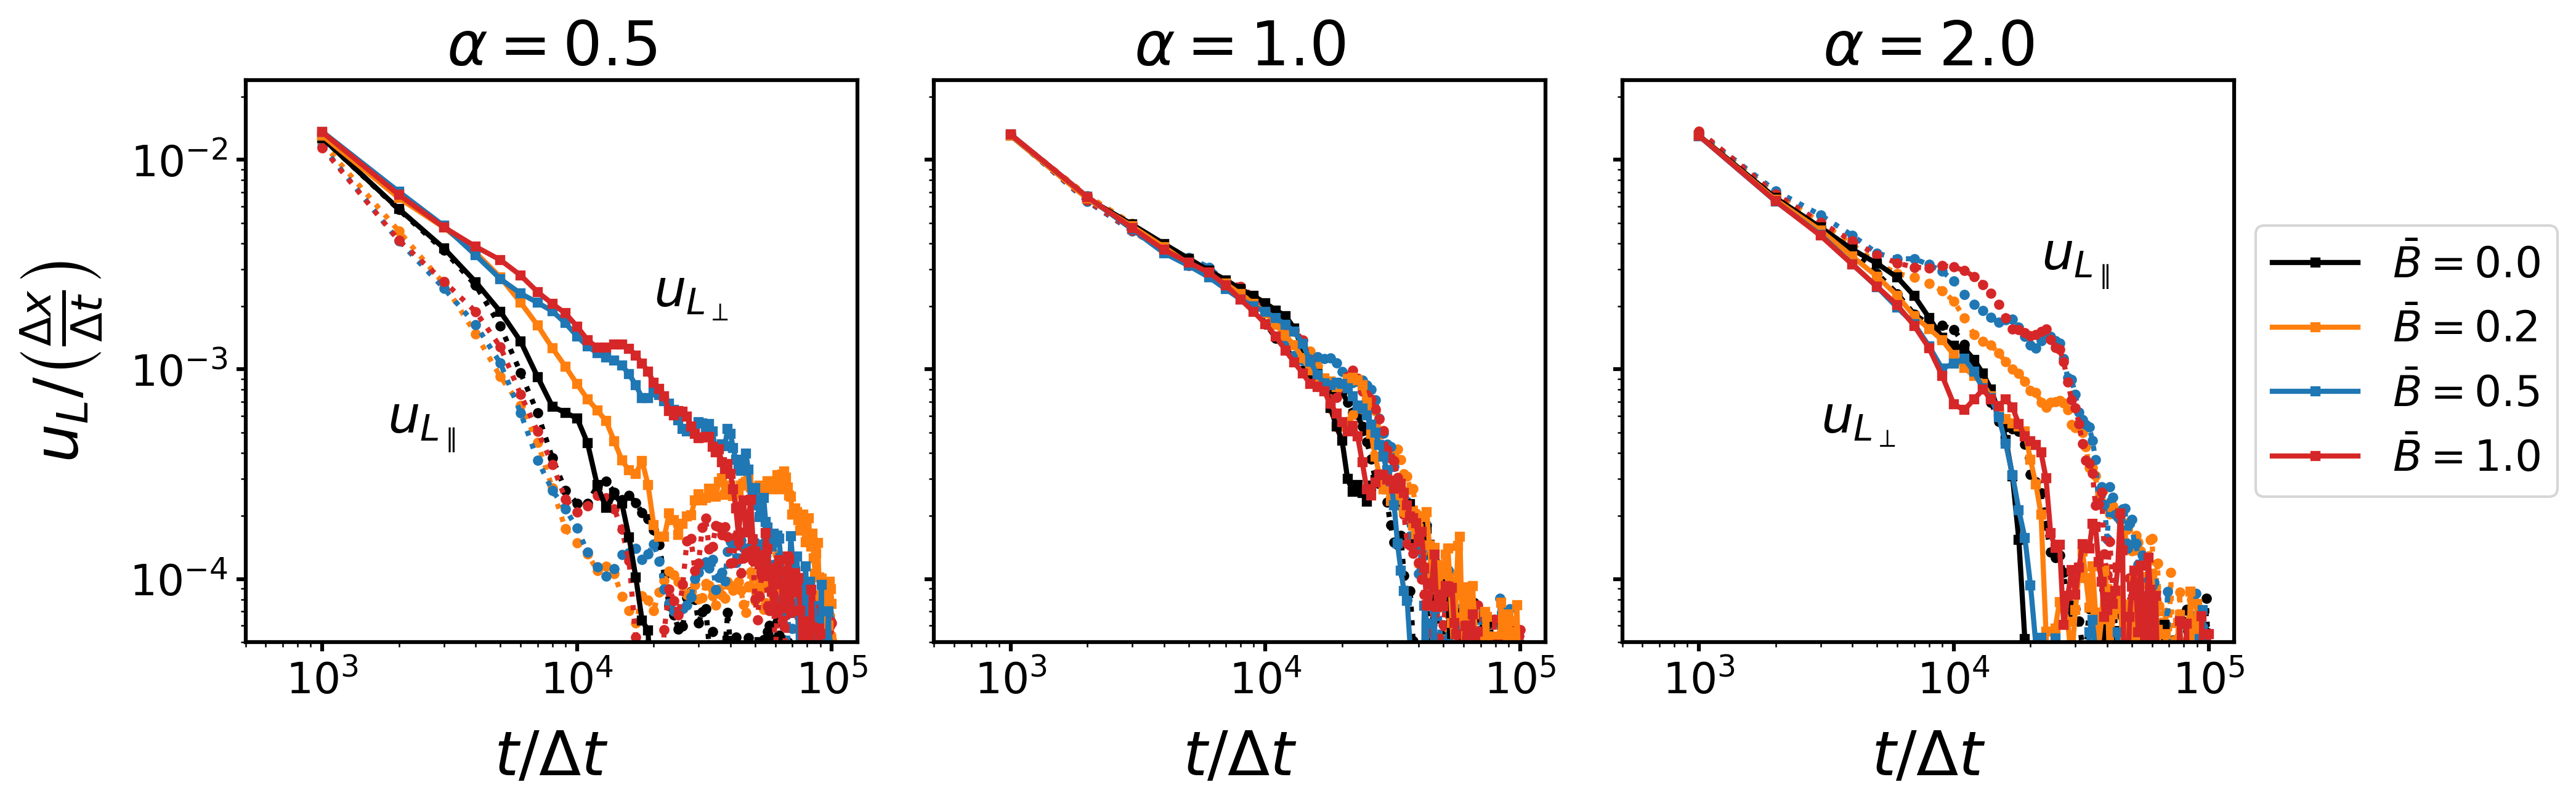
\includegraphics[width=\textwidth]{../figures/results/paper1/coarsening_vel.png}
    \caption{Time-dependence of the coarsening velocity $u_L$ for different particles shapes $\alpha$  and at different magnetic 
    field strength $\bar{B}$. The different components of the coarsening velocity show that the jamming time is different in the 
    direction parallel and perpendicular to the magnetic field.}
    \label{fig:coarsening_velocity}
    \end{figure*}
    
Figure~\ref{fig:coarsening_velocity} presents the coarsening speed along directions parallel and perpendicular to the applied magnetic field. For 
spherical particles, coarsening remains isotropic, as expected. The velocity is initially high but slows over time as particles begin to jam. 
Reeves et al.~\cite{reeves_particle-size_2015} emphasized the importance of the jamming time relative to the disruption time, where domain pinch-off can 
lead to depercolation and structural failure. However, in our simulations, we observe no such disruption—bijels remain stable across all conditions, in 
agreement with prior studies by Stratford et al.~\cite{stratford_colloidal_2005} and Jansen et al.~\cite{jansen_bijels_2011}.
    
In contrast, simulations with ellipsoidal particles show clear evidence of anisotropic coarsening in the presence of a magnetic field. For oblate 
particles (\(\alpha = 0.5\)), the coarsening speed increases in the direction perpendicular to the field as its strength grows, while the parallel 
direction remains largely unaffected. This suggests delayed jamming perpendicular to the field. Prolate particles show the opposite trend with coarsening 
accelerating along the field direction and jamming delayed relative to the perpendicular direction. Notably, we also observe a shoulder in the coarsening 
curve near \(10^4 \Delta t\), where the decay in speed slows before jamming occurs. 
    
These findings point to a magnetic field-dependent mechanism influencing coarsening near the jamming threshold. Specifically, the anisotropy appears 
linked to the reorientation and alignment of anisotropic particles with respect to the magnetic field. To test this hypothesis, we further examine the 
orientational order of particles and their alignment relative to both the field direction and the fluid interface.
    
\subsection{Particle re-orientation and packing}
    
    \begin{figure}
    \centering
    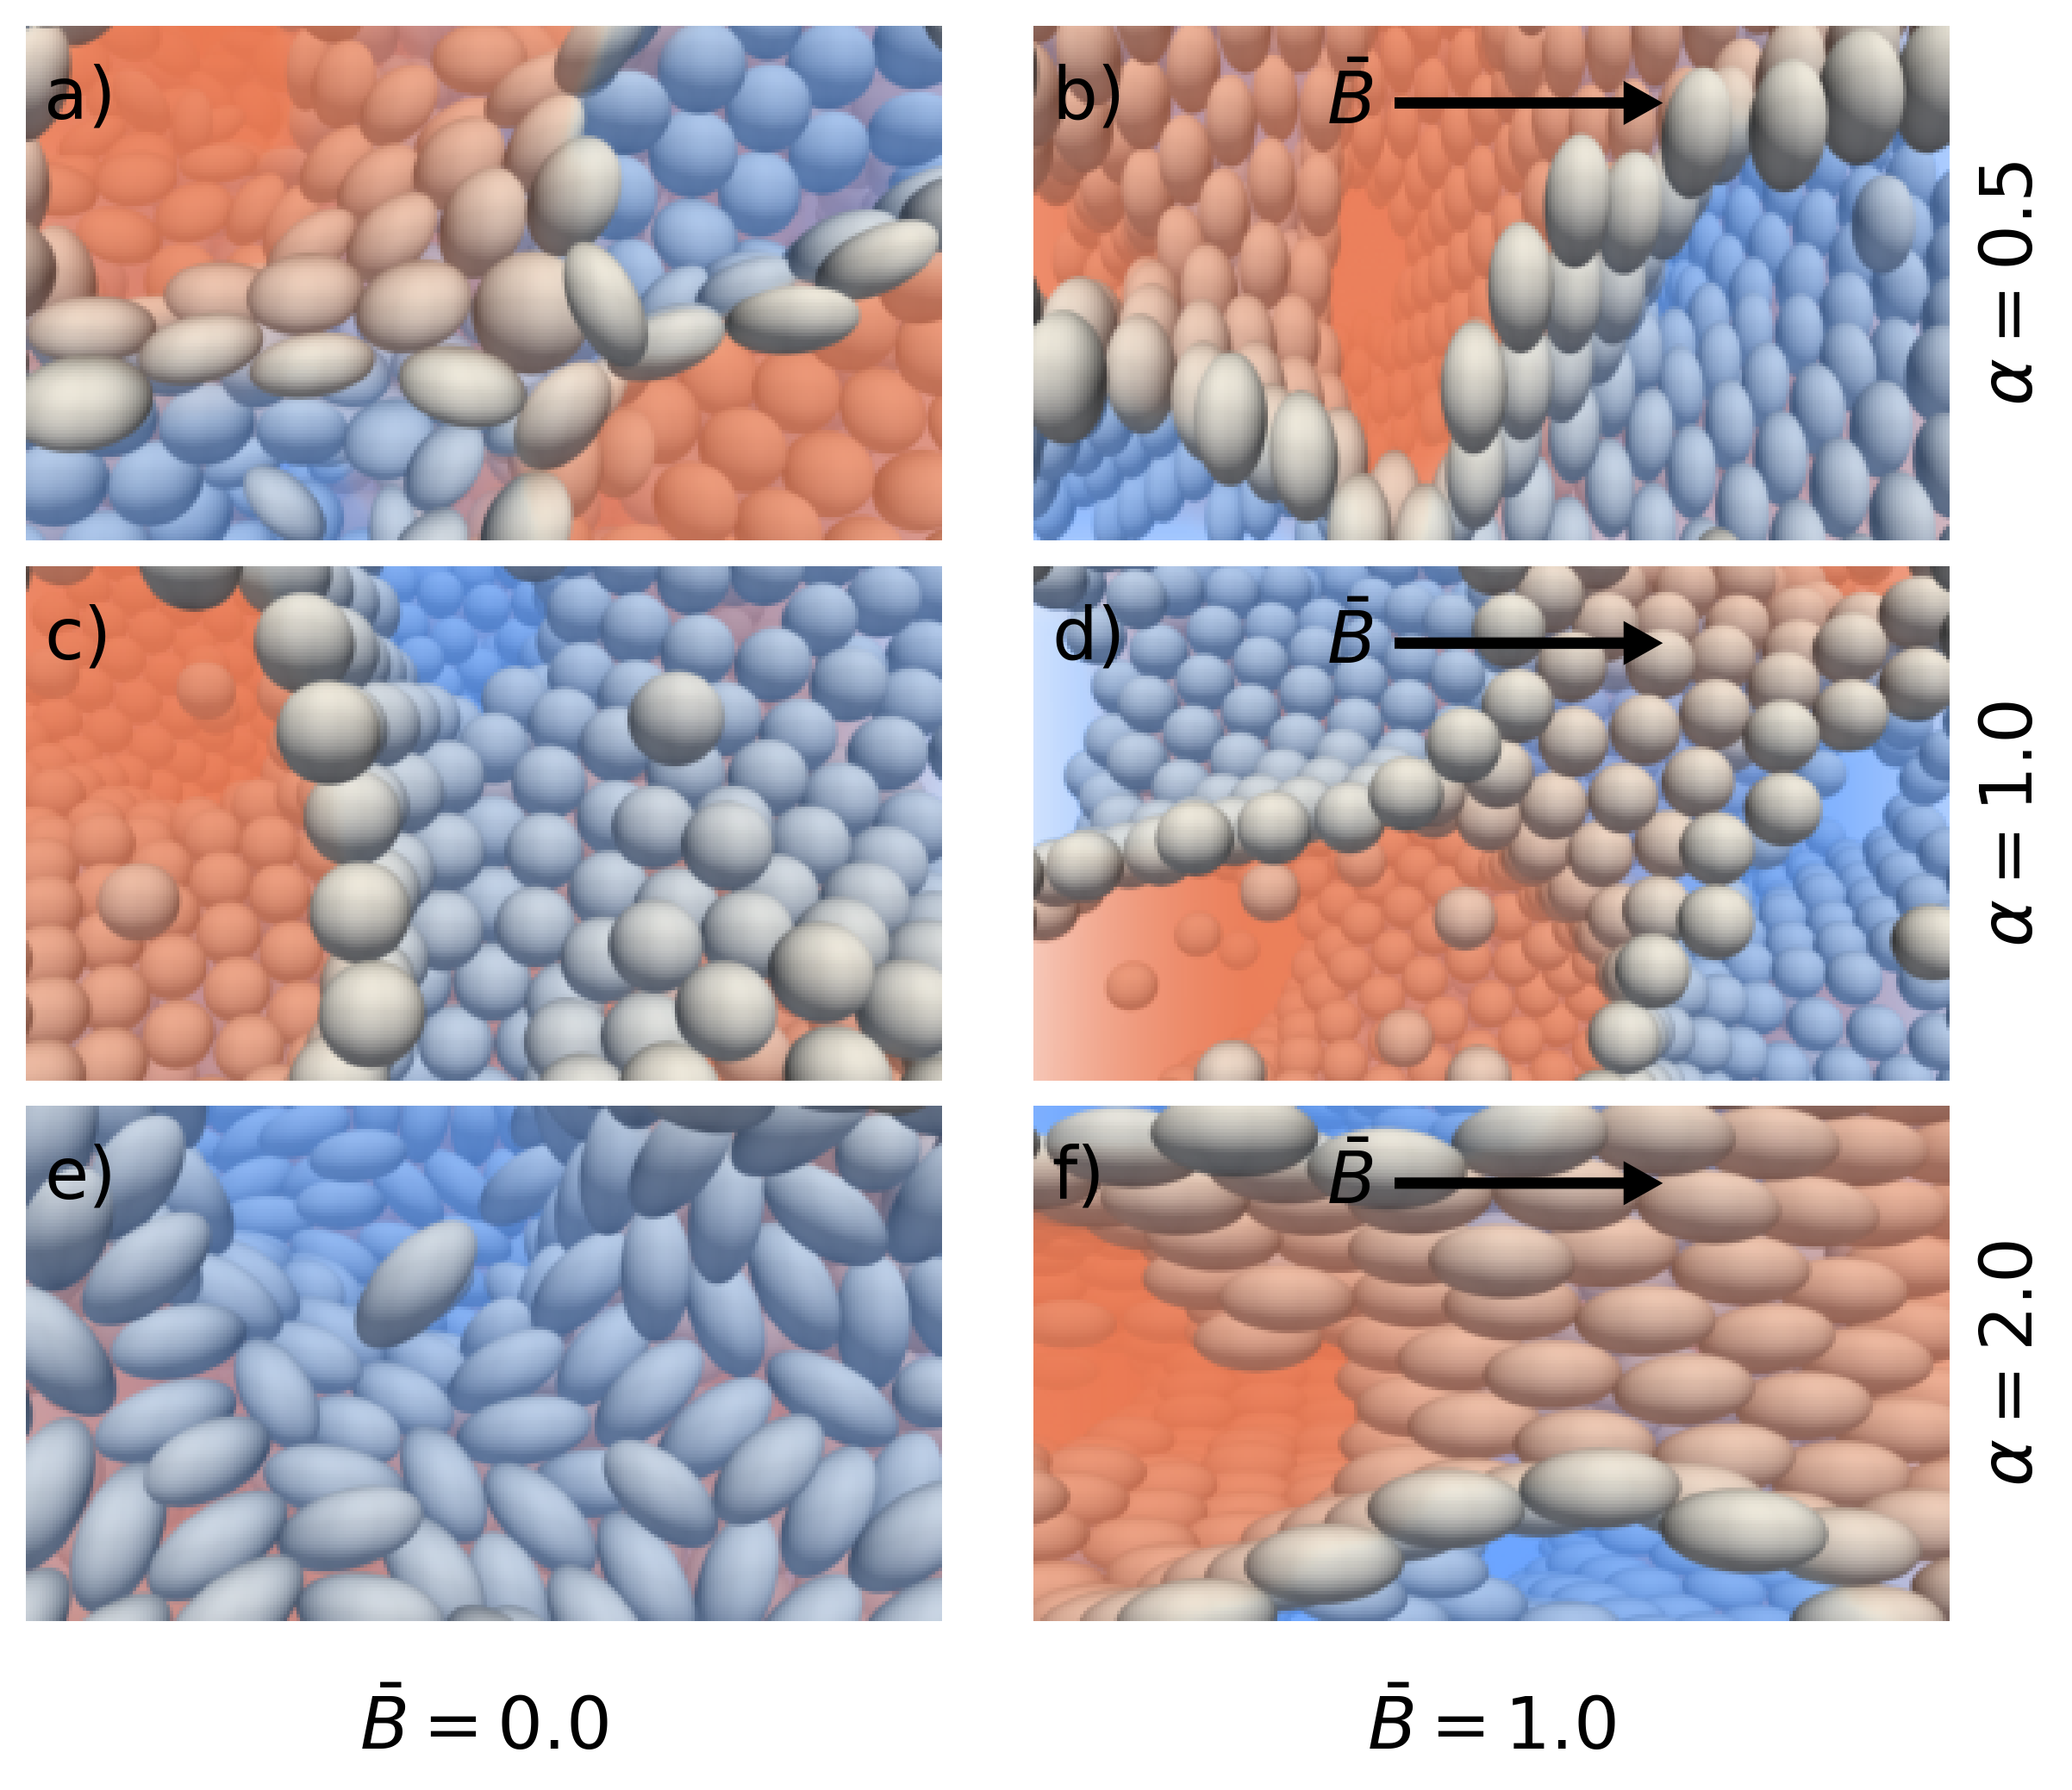
\includegraphics[scale=0.6]{../figures/results/paper1/particle_packing_viz.png}
    \caption{Snapshots illustrating the particle packing at the interface for different particle shapes $\alpha$ with (left)
     and without (right) applied magnetic field $\bar{B}$. The right column shows the alignment of the symmetry axis of the oblate (top row) and prolate (bottom row) 
     particles in the direction of the magnetic field indicated by arrows.}
    \label{fig:packing_viz}
    \end{figure}
    
The dominant influence of the magnetic field is the torque it applies to the particles magnetic dipoles, causing them to rotate and align with the 
field direction. This field-induced alignment is clearly visible in the simulation snapshots in Figure~\ref{fig:packing_viz}. In the absence of a 
magnetic field (\(\bar{B} = 0\)), the particles remain randomly oriented at the interface. When a magnetic field is applied (\(\bar{B} = 1\)), the 
dipoles exhibit pronounced orientational order aligned with the field. 

    
    \begin{figure}
    \centering
    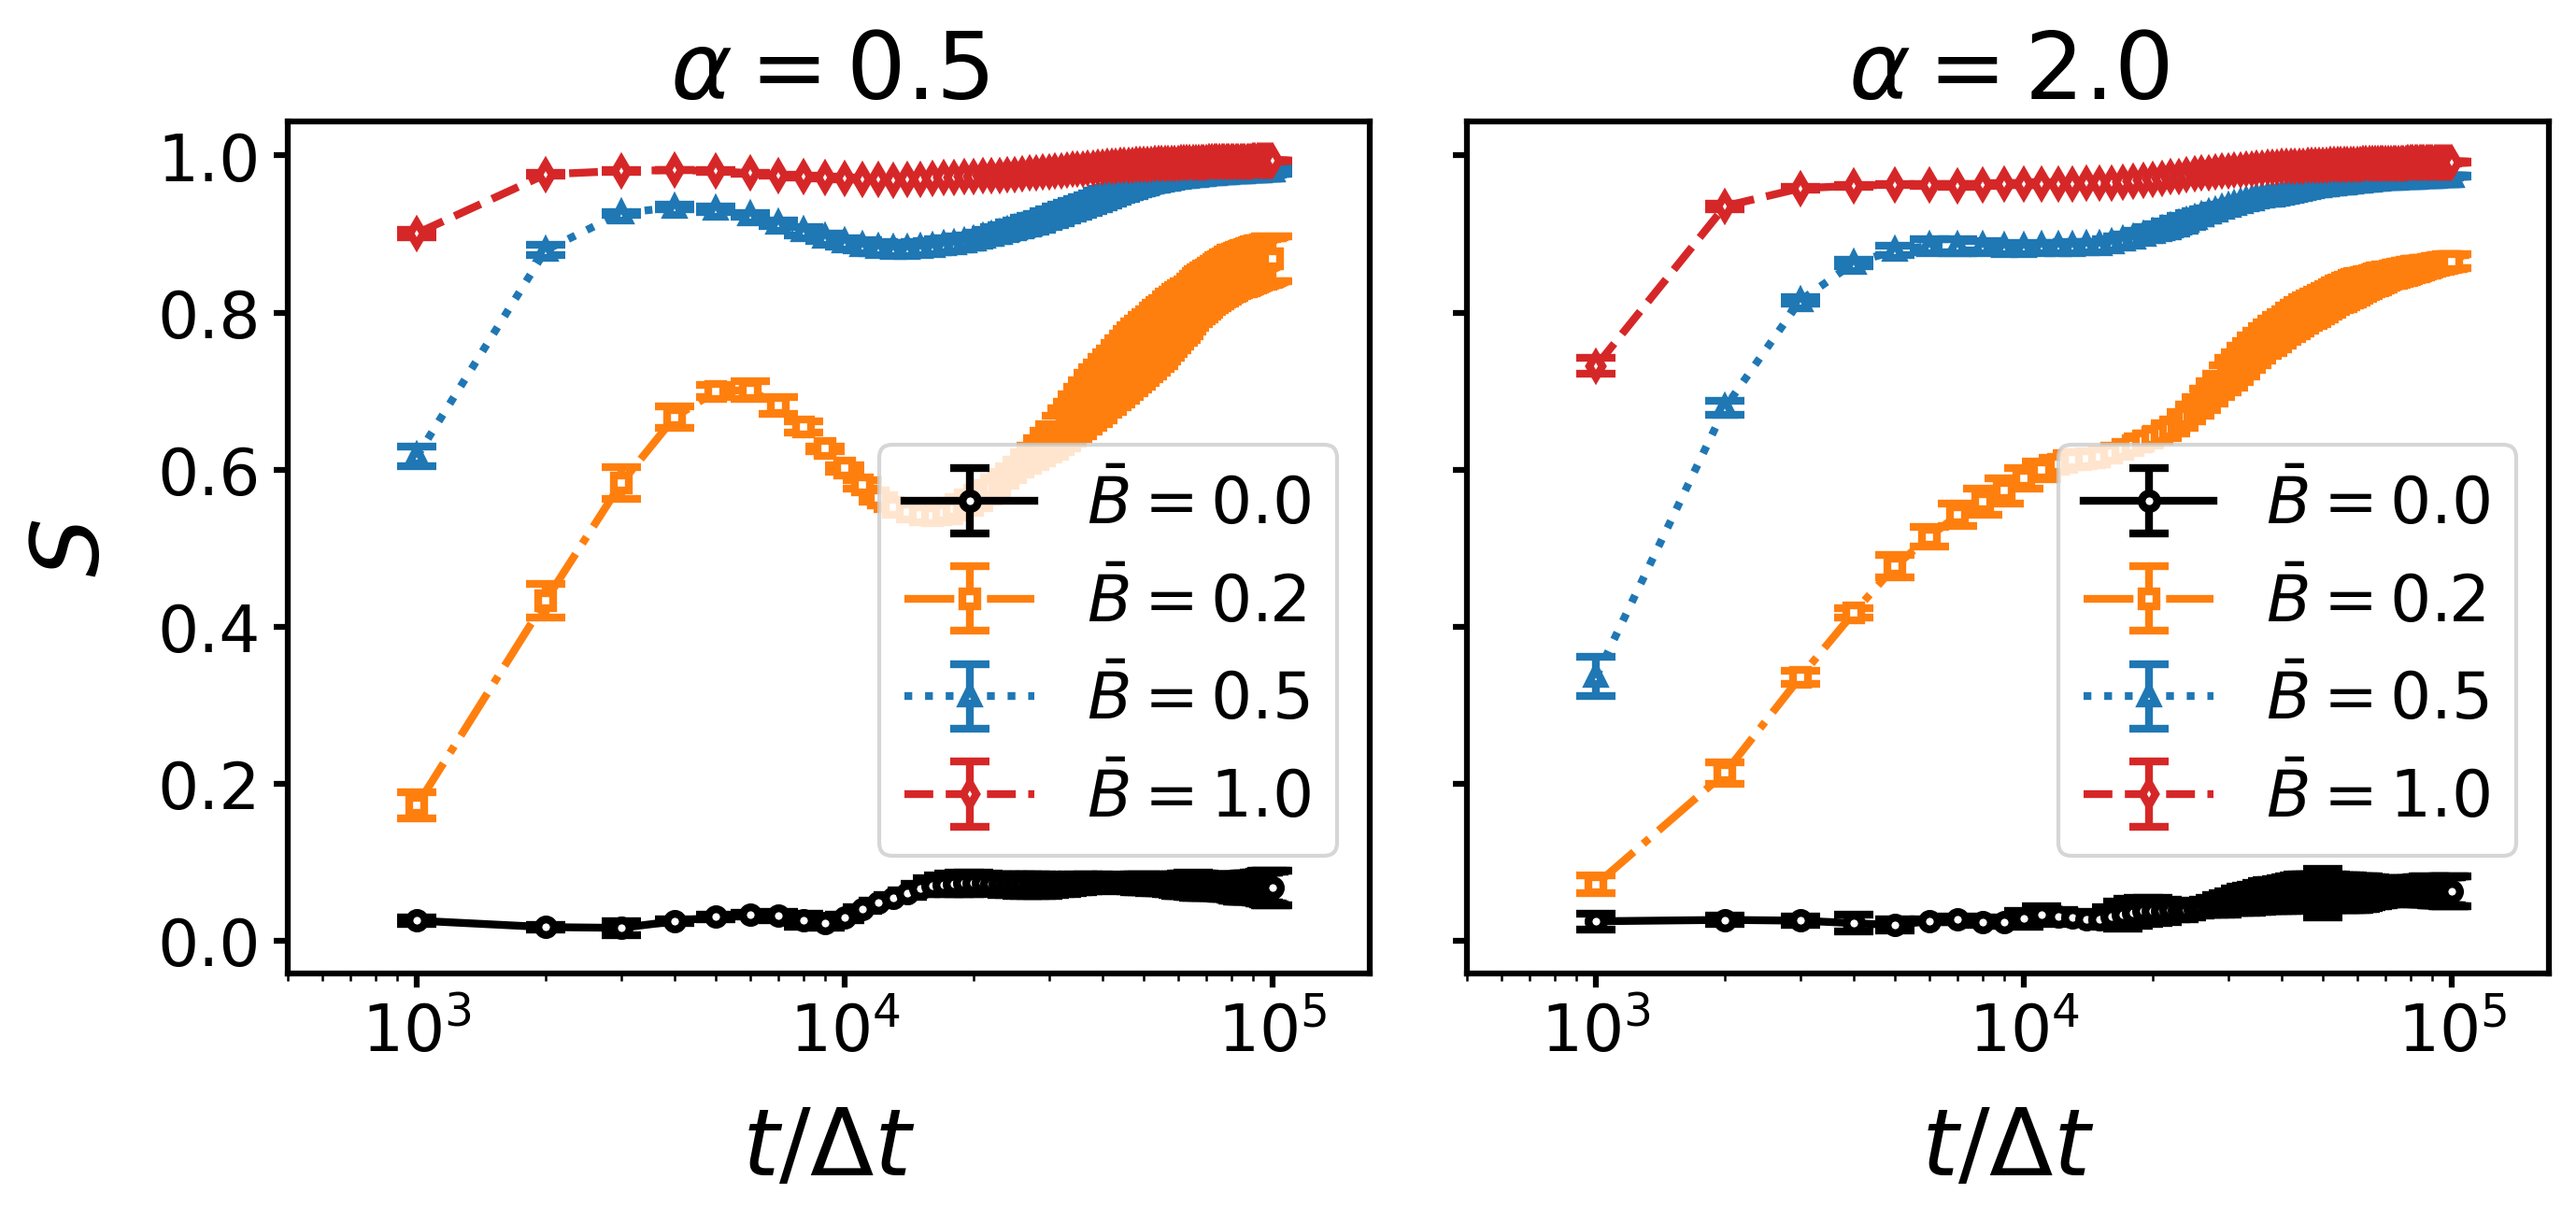
\includegraphics[scale=0.6]{../figures/results/paper1/S-vs-t.png}
    \caption{Time-dependence of the nematic order parameter $S$ of oblate ($\alpha=0.5$) and prolate ($\alpha=2$) particles at different field strength $\bar{B}$. Errorbars indicate the standard deviation taken over three independent simulation runs. Nematic order generally increases with applied field strength for all particle geometries. The increase slows down (for prolate particles) or reverses (for oblate particles) around $10^4$ timesteps.}
    \label{fig:nematic_time}
    \end{figure}
    
    To measure the particle alignment quantitatively, we computed the
    nematic order tensor \cite{veerman_phase_1992}
    %
    \begin{equation}
    \tens{Q} = \frac{1}{n_p} \sum_i \left( \frac{3}{2} \hat{\vec{o}}_i \otimes \hat{\vec{o}}_i -\frac{1}{2}\mathsf{1} \right) ,
    \end{equation}
    %
    where \(\hat{\vec{o}}_i\) is the orientation of the
    \(i\)-th particles and \(n_p\) is the number of particles in the system.
    The largest eigenvalue of \(\tens{Q}\) yields the nematic order
    parameter
    %
    \begin{equation}
    S = \left\langle \frac{3}{2}\cos^2 (\theta) - \frac{1}{2} \right\rangle ,
    \end{equation}
    %
    where
    \(\theta=\arccos(\hat{\vec{o}}_i\cdot\hat{\vec{n}})\) is the angle
    between the particle orientation and the nematic director
    \(\hat{\vec{n}}\).
    
Figure~\ref{fig:nematic_time} shows how the nematic order parameter \(S\) evolves over time for different particle aspect ratios \(\alpha\) and magnetic 
field strengths \(\bar{B}\). The onset of orientational order is nearly immediate and increases with field strength. For \(\bar{B} \ge 0.5\), \(S\) 
approaches saturation at around 1.0 by the end of the simulation. In the case of prolate particles (\(\alpha = 2.0\)), a shoulder appears around 
\(10^4 \Delta t\), forming a temporary plateau. This behavior coincides with the slower decline in coarsening speed seen in 
Figure~\ref{fig:coarsening_velocity}. For oblate particles, the effect is even more pronounced—\(S\) exhibits an intermittent drop before rising again.
    
These fluctuations in orientational order align with the delayed jamming observed in directions perpendicular (oblate) and parallel (prolate) to the 
magnetic field. The underlying mechanism appears to be the early alignment of particles with the field, which reduces steric hindrance at the interface 
and allows further coarsening. However, as the interface evolves, reorientation can induce capillary torques that compete with the magnetic torque, 
temporarily disrupting the nematic alignment. This competition explains the observed dips and plateaus in \(S\), particularly at lower field strength 
(\(\bar{B} = 0.2\)), where the decay is most pronounced.
    
To further corroborate this mechanism, we quantify the orientational, order of the interfaces. We computed the interfacial orientation tensor
    %
    \begin{equation}
    \tens{Q}_{\text{int}} = \frac{1}{\langle \mathrm{tr}(\tens{A}) \rangle} \left\langle \tens{A} - \frac{1}{3} \mathrm{tr}(\tens{A}) \mathsf{1} \right\rangle ,
    \end{equation}
    %
where the local tensor field \(\tens{A}\) is defined by
    %
    \begin{equation}
    \tens{A} = \nabla \phi \otimes \nabla \phi .
    \end{equation}
    %
The largest eigenvalue of \(\tens{Q}\) is taken as the interface nematic order parameter $S_{\text{int}}$.
    
    \begin{figure}
        \centering
    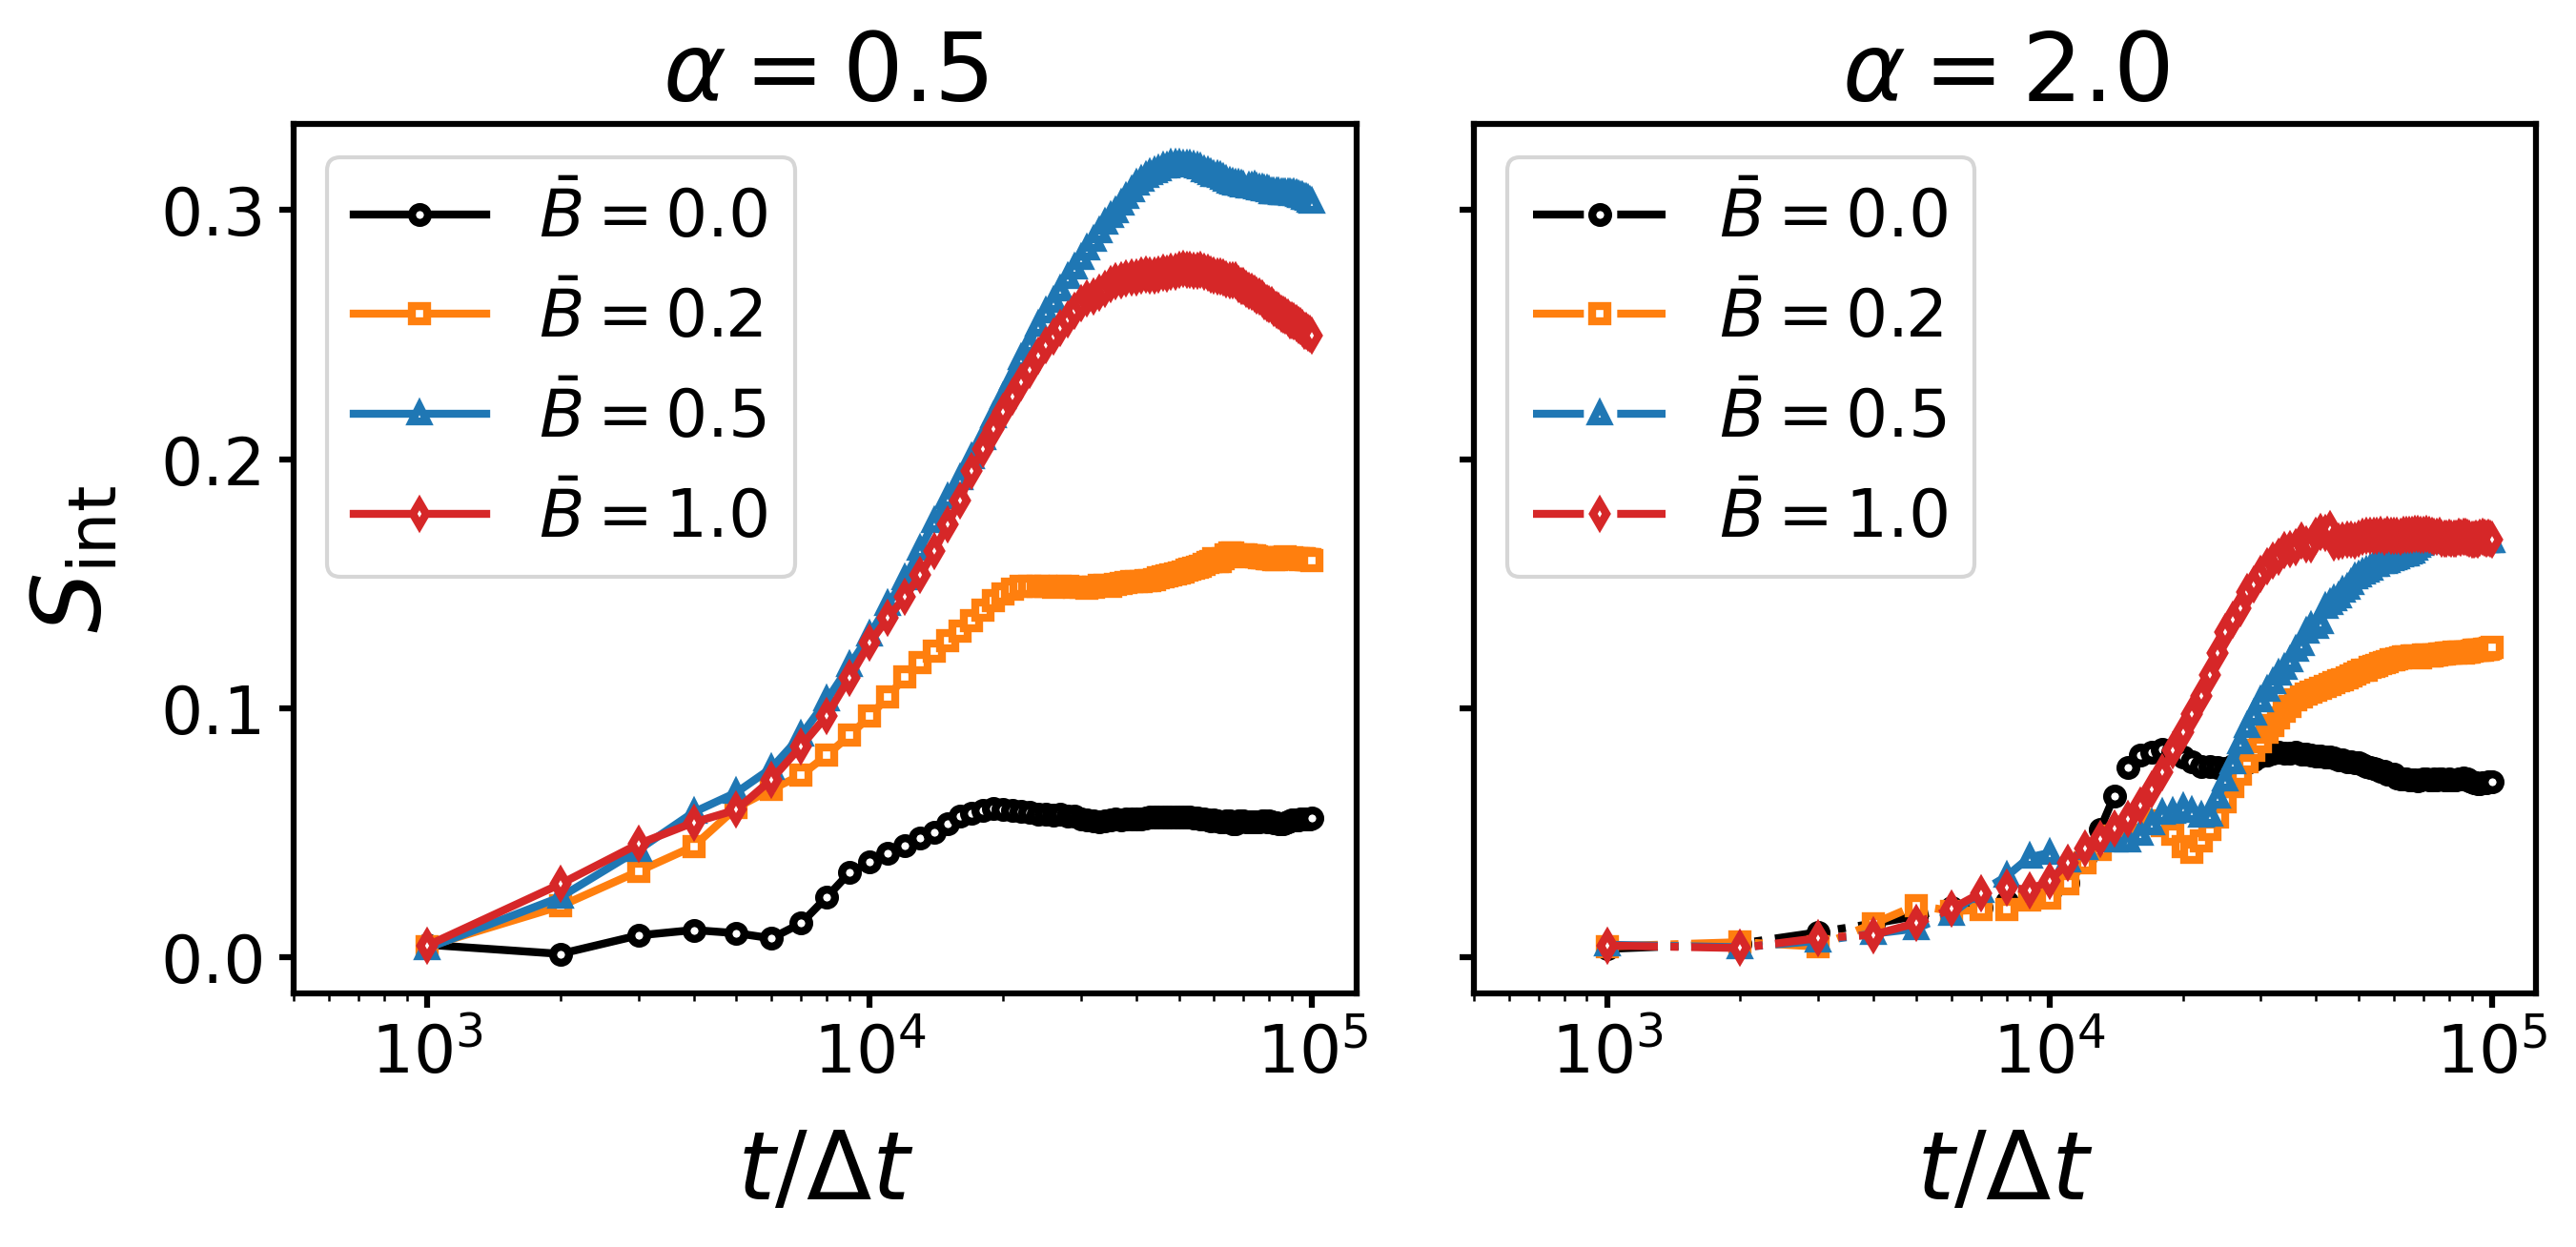
\includegraphics[scale=0.6]{../figures/results/paper1/interface_nematic.png}
    \caption{Time-dependence of the interface nematic order for oblate ($\alpha=0.5$) and prolate ($\alpha=2$) particles at different magnetic field strength $\bar{B}$. The interface alignment tends to increase with increasing field strength. The rate of increase becomes larger around $10^4$ timesteps, indicating the alignment of the interfaces due to capillary interactions with the particles.}
    \label{fig:interface_nematic}
    \end{figure}

Figure~\ref{fig:interface_nematic} presents the evolution of the interface nematic order parameter \(S_{\text{int}}\). Interface alignment increases over 
time, with higher magnetic field strengths \(\bar{B}\) accelerating this process. In all cases, \(S_{\text{int}}\) remains below 0.5 by the end of the 
simulation, indicating that the interface retains its tortuous, bicontinuous morphology despite the field. This confirms that particle reorientation promotes 
partial alignment without disrupting the overall bijel structure.
    
As particles rotate, they experience a capillary torque from the interface due to surface tension and contact angle constraints. If the magnetic torque 
surpasses this, particles may overcome the capillary barrier and tilt out of the interface. For prolate particles (\(\alpha = 2\)) at flat interfaces, 
Davies et al. showed that a transition from flat to tilted orientation occurs at a critical field strength of \(\bar{B} \approx 0.2\) 
\cite{bresme_orientational_2007,davies_interface_2014,newton_influence_2014}. In bijels, however, the interfaces are curved and mobile. We propose that 
instead of tilting out, particles “drag” the interface as they rotate, guiding alignment of the surrounding liquid domains. For anisotropic particles, 
we expect this alignment to occur perpendicular to the symmetry axis in oblates and parallel in prolates. The previously discussed domain size and 
tortuosity data support this assumption.
    
To verify that particles maintain their preferred orientation relative to the interface, we analyzed the angle between each particles symmetry axis and 
the local interface normal. We generated a mesh of the interface using the marching cubes algorithm and, for each particle, identified the nearest mesh vertex 
(excluding those beyond the length of the particle's long axis). We then calculated the angle \(\psi\) between the particle orientation vector 
\(\hat{\vec{o}}_i\) and the local surface normal. The time evolution of the average angle \(\psi\) is shown in Figure~\ref{fig:psi_time}.
    
\begin{figure}
    \centering
    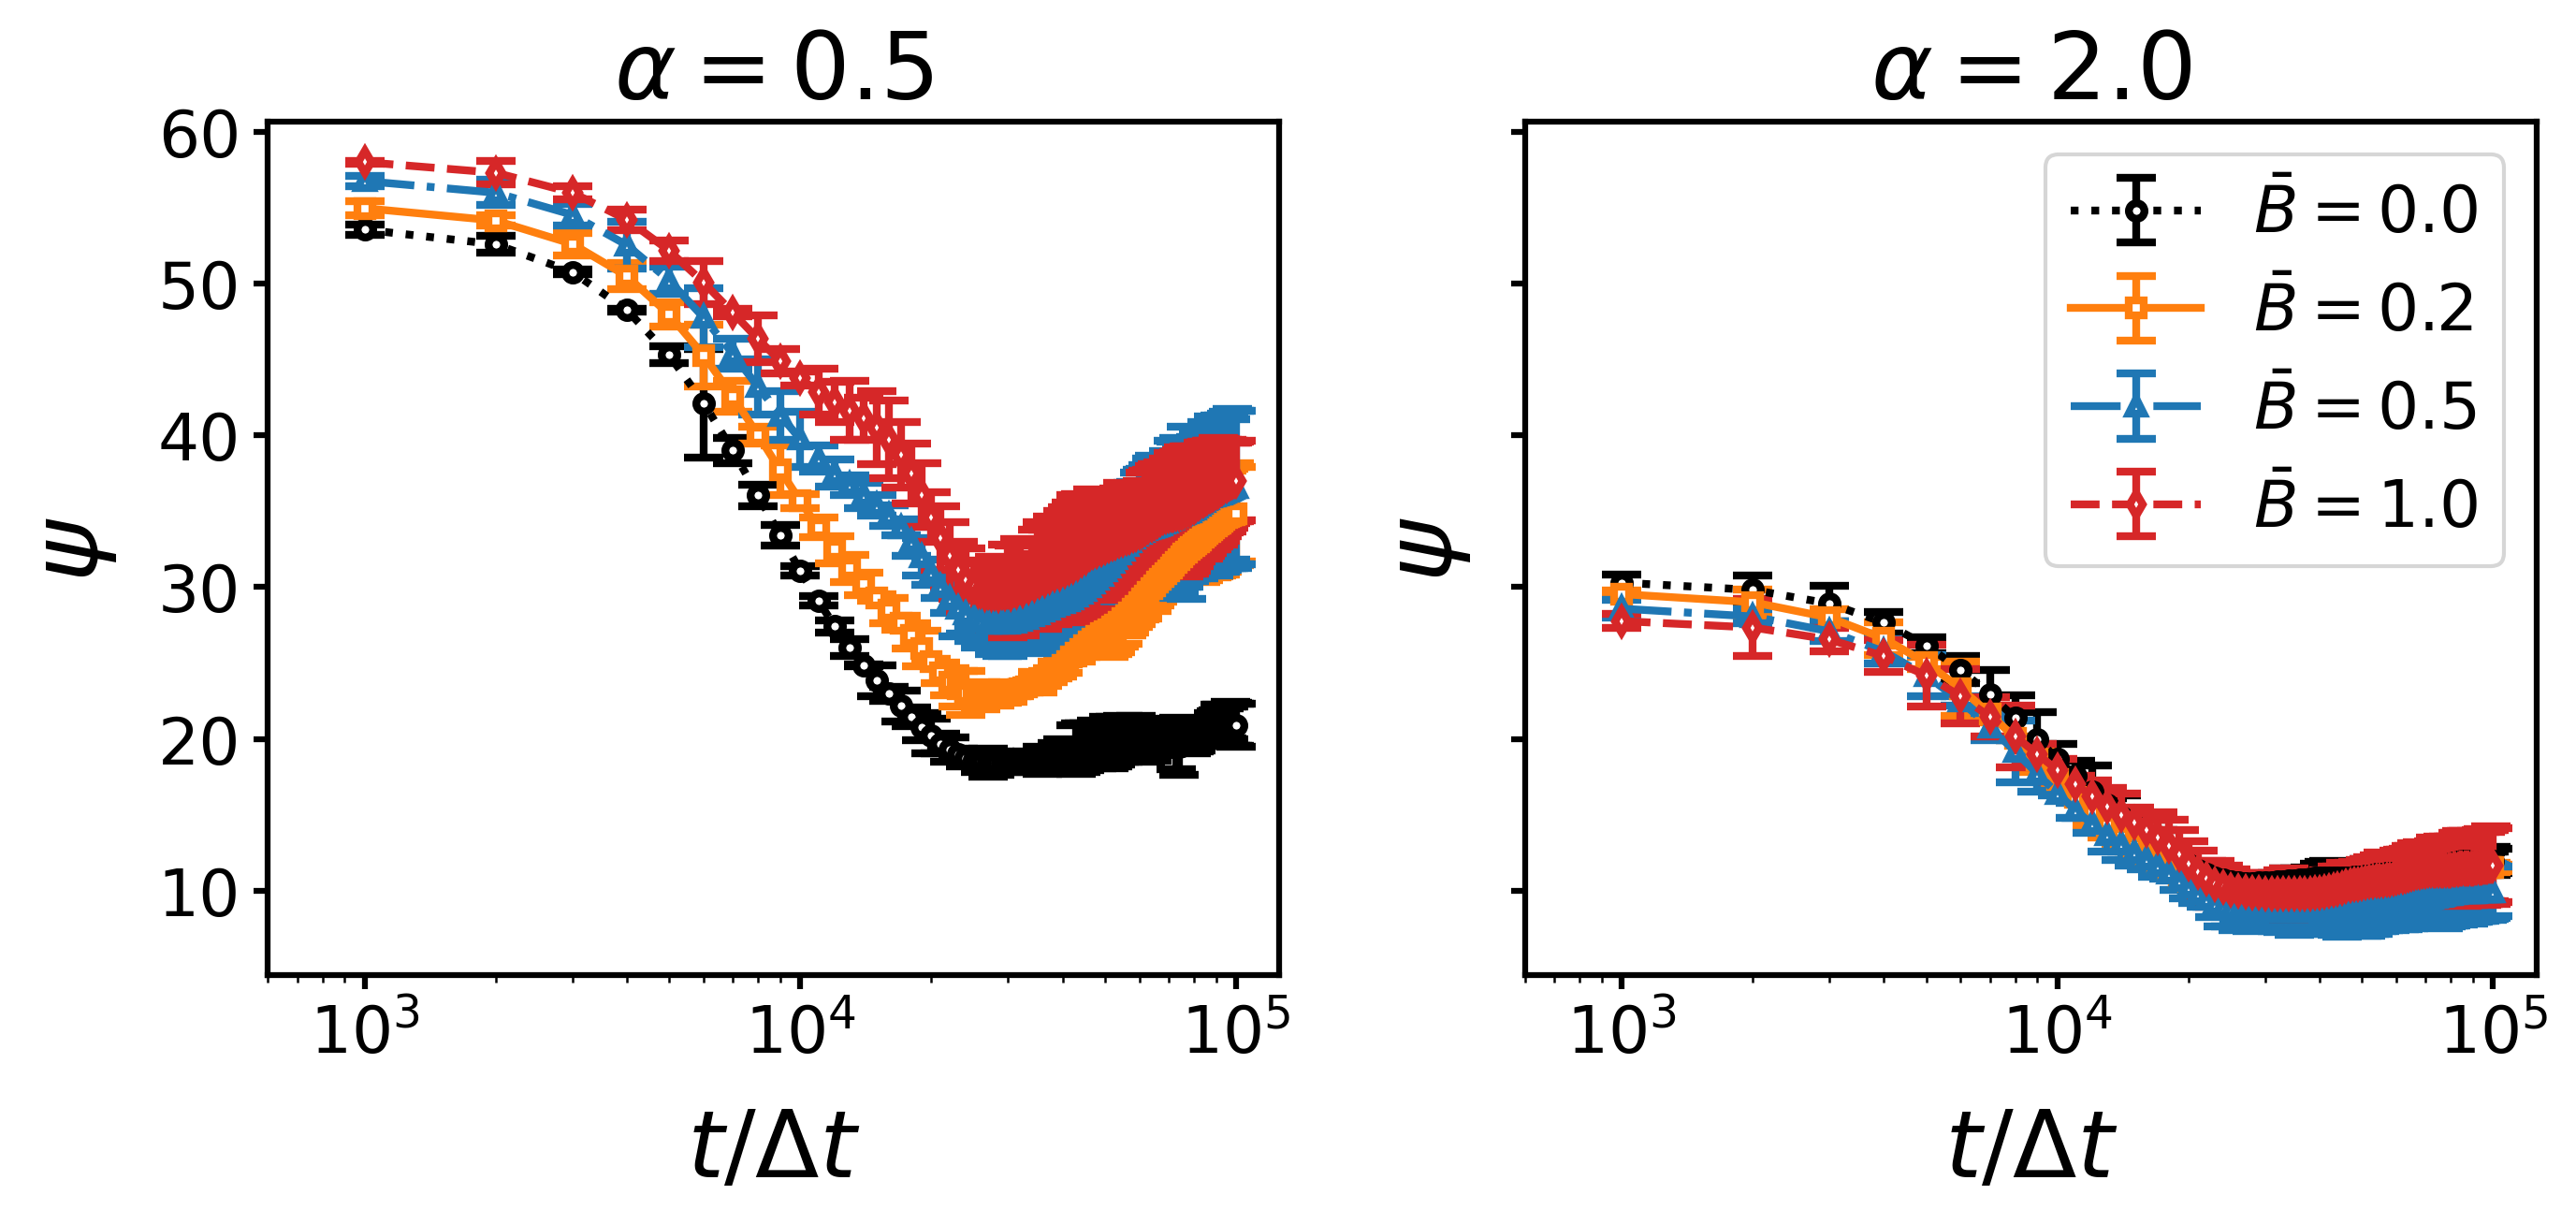
\includegraphics[scale=0.6]{../figures/results/paper1/psi-vs-t.png}
    \caption{Time-dependence of the average angle $\psi$ between the particle axis and the interface normal for oblate ($\alpha=0.5$) and 
             prolate ($\alpha=2$) particles at different magnetic field strength $\bar{B}$. Errorbars indicate the standard deviation taken over 
             three independent simulation runs. The angle between between the particles and the interface normal generally approaches the energetically 
             preferred value ($0^\circ$ for oblate particls, $90^\circ$ for prolate particles). The average angle changes most rapidly around $10^4$ timesteps.}
\label{fig:psi_time}
\end{figure}
    
For both types of anisotropic particles, the initial angle between the particle dipole and the interface normal is approximately 
\(\psi \approx 60^\circ\). As the spinodal interface propagates through the system, particles attach and begin aligning due to capillary torque. 
In oblate particles, this results in alignment of the dipole axis with the interface normal, reflected by a decrease in \(\psi\) toward zero. In 
contrast, prolate particles preferentially align their dipole axis parallel to the interface, causing \(\psi\) to increase toward \(90^\circ\).
    
The most significant changes in \(\psi\) occur around \(10^4 \Delta t\), coinciding with notable features in coarsening speed and particle nematic 
order discussed earlier. These trends support the proposed mechanism of particle reorientation under magnetic fields and the associated local 
alignment of the interface. As jamming begins and the available interfacial area decreases, some particles are pushed out of their preferred 
alignment. This leads to an increase in \(\psi\) for oblate particles and a decrease for prolate particles.

Figure~\ref{fig:psi_time} suggests that this forced misalignment is more pronounced for oblate particles. Due to their larger aspect ratio, prolate 
particles experience stronger capillary torques when tilted, making them more resistant to reorientation. As a result, prolate particles largely 
maintain alignment with the interface, even under stronger magnetic fields.

As hypothesized above, the alignment of the particle dipole axis with
the magnetic field reduces the steric constraints within the interface.
To corroborate this idea, we analyzed the radial distribution function
(RDF) of the particles
    %
    \begin{equation}
        g(r) = \frac{n_p - 1}{n_p} \cdot V \cdot \left\langle \delta\left(r - r_i\right) \right\rangle
    \end{equation}
    %
where \(n_p\) is the number of particles in the volume
\(V\), and \(\langle\cdot\rangle\) denotes an average over all
particles. The radial distribution function was calculated by binning
the distance between all particle pairs and normalizing the shells with
respect to the distribution \(4\pi \rho r^2 \mathrm{d}r\) of an ideal
gas. The time-evolution of the RDFs for the three particle shapes and
varying magnetic flux density is illustrated in Figure \ref{fig:rdf}.
    
    \begin{figure*}
    \centering
    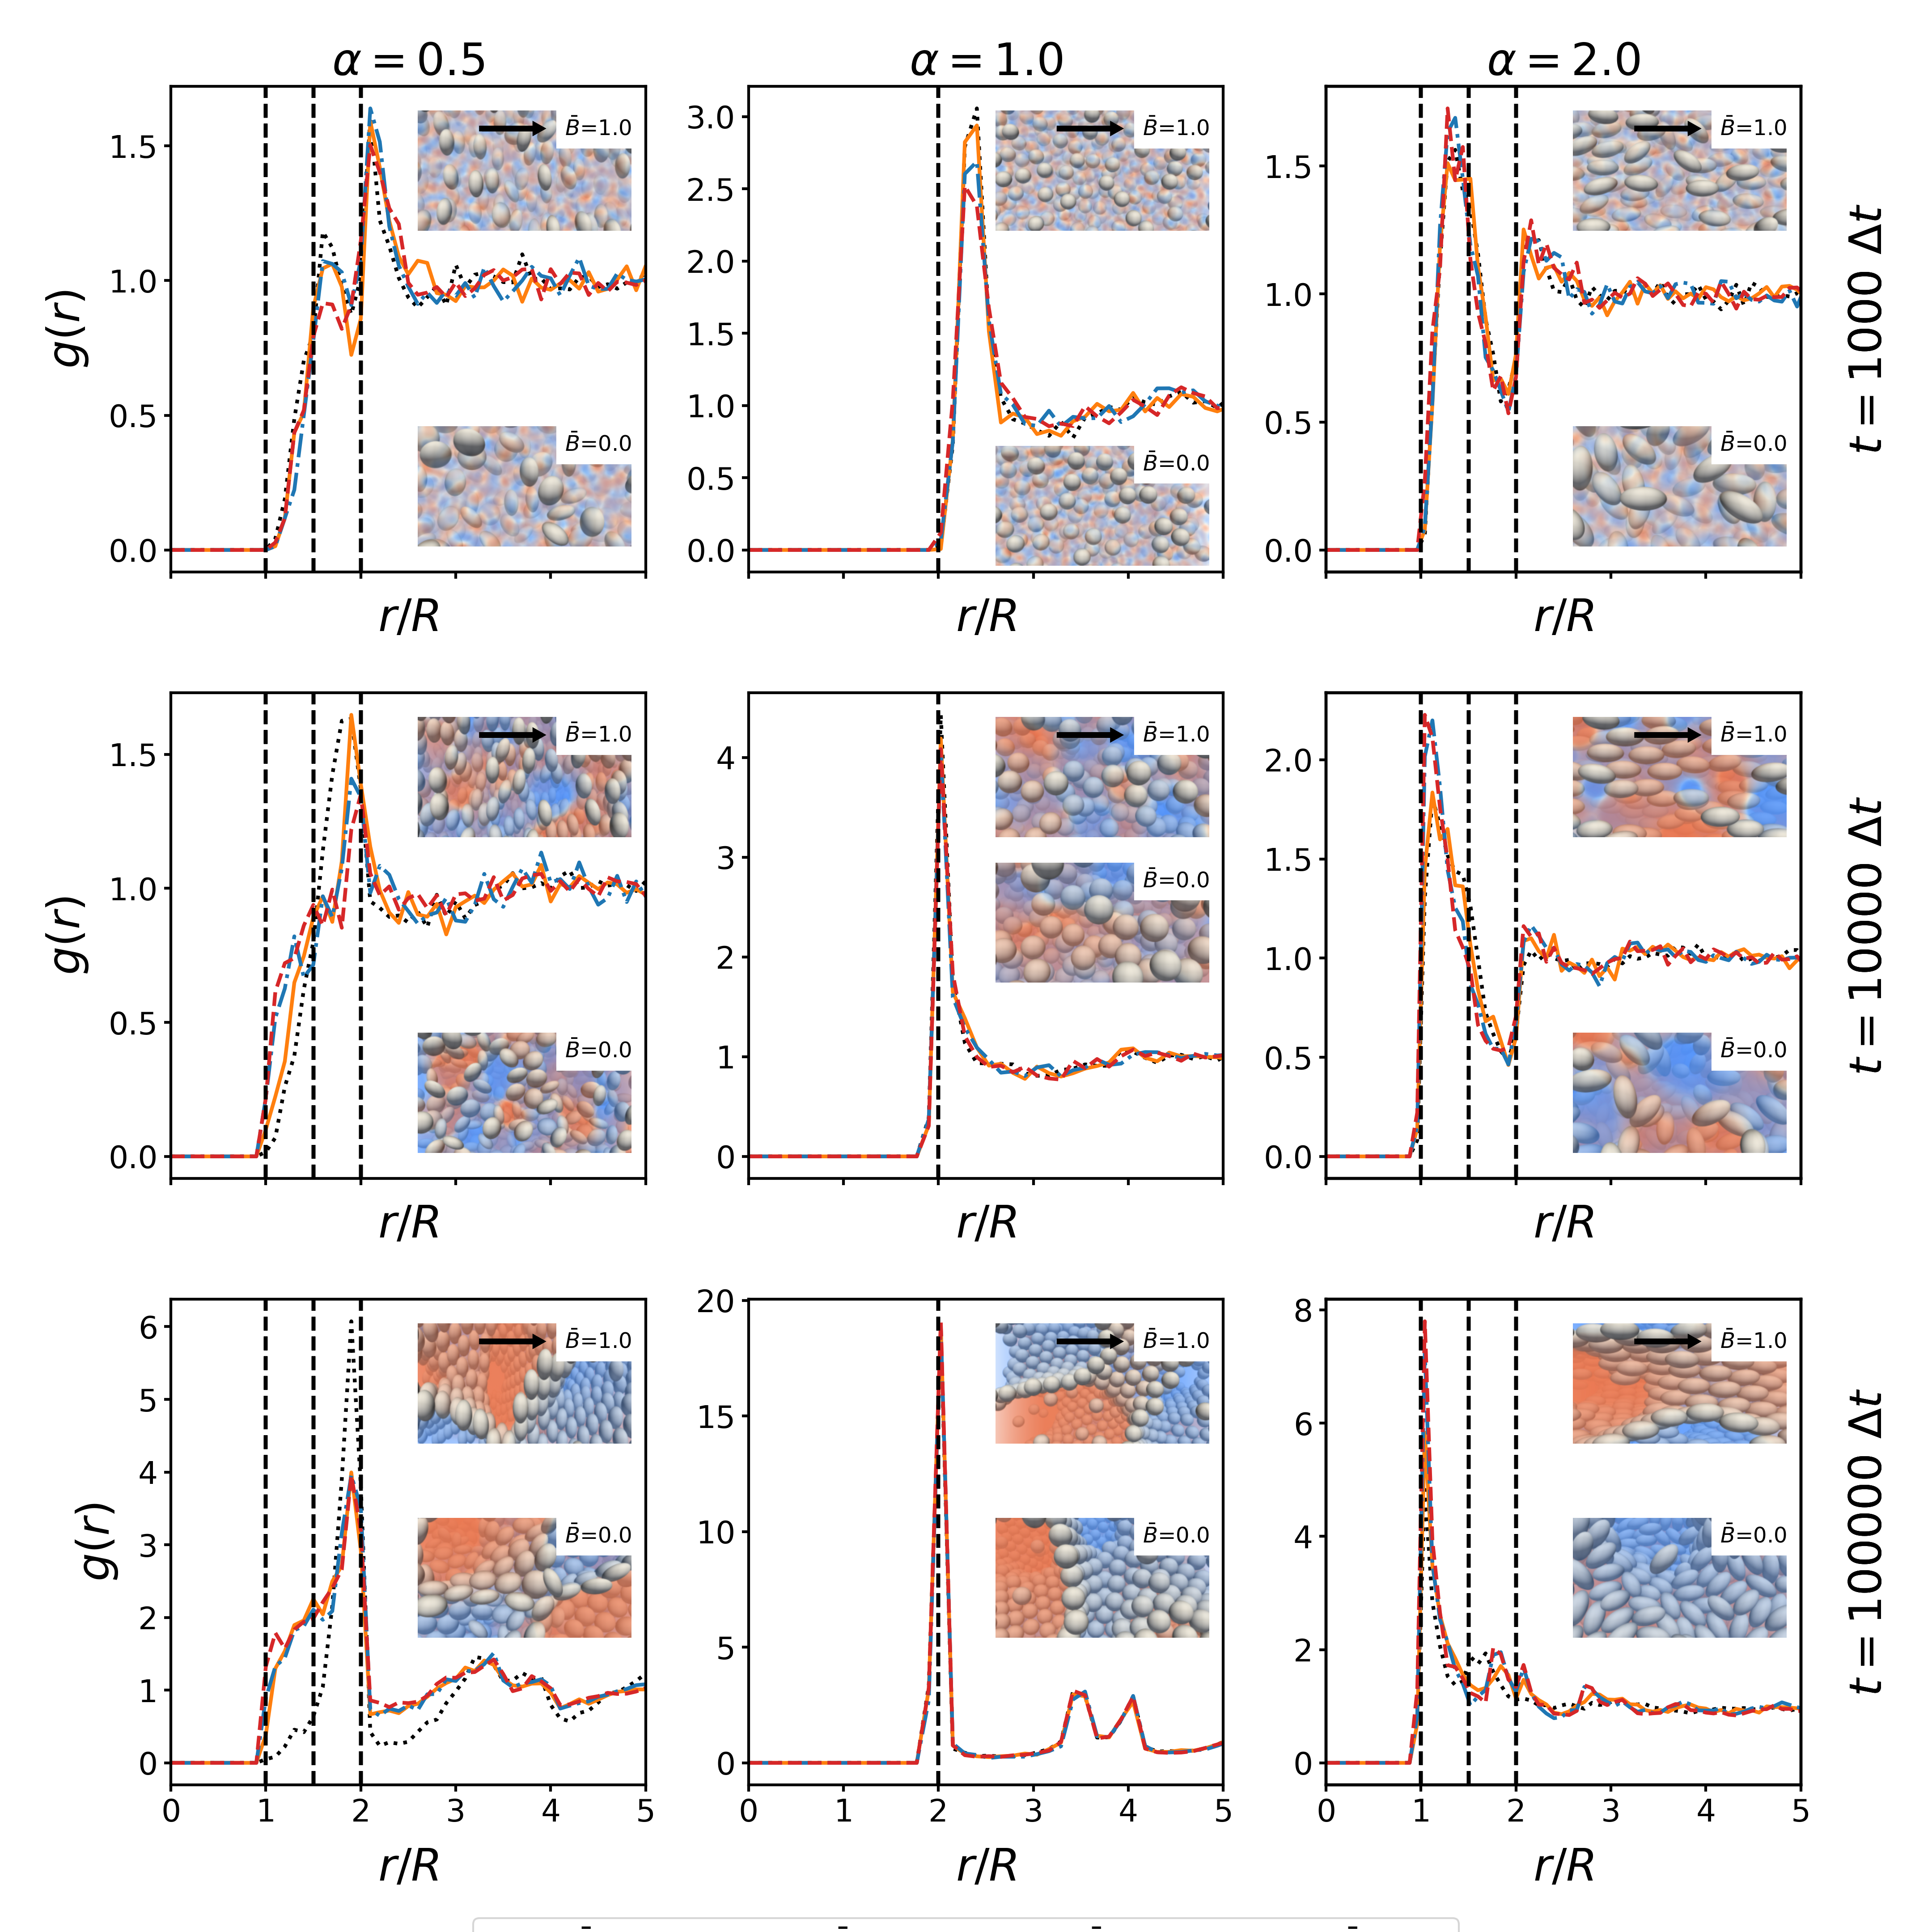
\includegraphics[scale=0.4]{../figures/results/paper1/rdf_compare_time.png}
    \caption{Time-evolution of the radial distribution function $g(r)$ of the particles at different magnetic field strength $\bar{B}$. The radial 
    distribution function is shown at $10^3$, $10^4$, and $10^5$ timesteps. The distance $r$ is normalized by the radius $R=\max(R_\parallel,R_\perp)$ 
    of the larger particle axis. The peaks illustrate the packing of particles in the interface. Dashed lines indicate the side-by-side, tip-to-tip, and 
    side-to-tip configuration of particle pairs. For spherical particles, the three values are identical.}
    \label{fig:rdf}
    \end{figure*}

Figure~\ref{fig:rdf} shows the radial distribution function (RDF) at time steps $t = 1000\Delta t, 10000\Delta t, 100000\Delta t$. 
For ellipsoidal particles, characteristic contact distances include \(2R_{\parallel}\), \(2R_{\perp}\), and \(R_{\parallel} + R_{\perp}\), 
indicated by dashed lines in the figure. The largest RDF peak for both oblate and spherical particles occurs at \(2R_\perp\), suggesting 
contact around the particle circumference, while prolate particles preferentially align side-by-side. These configurations enable denser 
packing at the interface.

In the early stages of the simulation, RDF peaks are less distinct due to the more random particle orientations. Notably, for prolate particles, 
the RDF shows an initial dip at \(2R_\parallel\), indicating that tip-to-tip arrangements are rare. As time progresses, the peak heights increase, 
particularly under magnetic fields, supporting the idea that magnetic alignment promotes side-by-side and tip-to-tip ordering. For oblate particles, 
a shoulder emerges near \(R_\parallel + R_\perp\), indicating occasional tilting out of the interface to reduce interfacial coverage. In contrast, 
for prolate particles, the dip at \(2R_\parallel\) disappears over time, suggesting increased tip-to-tip alignment, consistent with field-driven 
particle orientation that supports close packing along both particle axes. This layered structure is also visible in the snapshots in 
Figure~\ref{fig:packing_viz}.

Together with the nematic order analysis, these findings reinforce the proposed mechanism of bijel formation under magnetic fields: the field aligns 
particle dipoles, particle reorientation couples to interface alignment via capillary interactions, and steric constraints are reduced, allowing further 
interface shrinkage and domain coarsening. Temporally, particle rotation occurs early in the simulation, followed by gradual re-alignment of interfaces. 
For prolate particles, shrinking interfaces can even force slight misalignment to accommodate tighter packing. Overall, our results demonstrate that 
bijels formed under magnetic fields with anisotropic particles develop anisotropic domain sizes and tortuosity, and exhibit more ordered interfacial 
particle packing due to alignment effects.
    
\section{Conclusions}

In this work, we investigated how external magnetic fields affect the formation of bijels stabilized by magnetic ellipsoidal particles. We considered 
oblate, spherical, and prolate particles with permanent magnetic dipoles dispersed in a symmetric binary fluid. While the presence of a magnetic field 
does not prevent bijel formation, it induces anisotropy in both domain size and tortuosity when using non-spherical particles. For oblates, domain size 
increases perpendicular to the field, while tortuosity increases along the field direction. In contrast, for prolates, domain growth is enhanced along 
the field, with increased tortuosity perpendicular to it. Compared to bijels formed without a field, domain size changed by up to 30\% for anisotropic particles.

This behavior is driven by particle reorientation: magnetic dipoles align with the field, which in turn influences interface alignment along the longer axis 
of the particles. Our analyses of coarsening velocity, nematic ordering, and interfacial structure support this mechanism. We observed that jamming is delayed 
in the direction aligned with the particles long axis, allowing extended coarsening. This delay correlates with a slowdown in particle alignment and increased 
interface ordering. We also found that the average angle between particle dipoles and the interface normal evolves during this stage. Radial distribution 
functions further show that prolate particles tend to align side-by-side, while oblates form less regular arrangements.
Together, these findings suggest that bijel formation under magnetic fields is governed by two coupled processes: initial magnetic alignment of the particles, 
which facilitates coarsening, followed by capillary-induced interface alignment. As jamming sets in, interfacial shrinkage compresses particles into ordered 
structures. Some particles, particularly oblates, may tilt out of the interface to accommodate tighter packing.

Our results highlight how magnetic fields can be used to tune the structural properties of bijels, which is valuable for applications where domain size and 
tortuosity affect performance. For instance, reduced tortuosity can enhance diffusive transport in bone-like materials \cite{prakoso2023tortuosity} and 
lithium-ion electrodes \cite{chen2020tortuosity, ebner2014tortuosity}, improving efficiency and cyclability. While we focused on a specific spinodal 
decomposition regime, further tuning could be achieved by adjusting fluid viscosity, surface tension, or particle volume fraction, known to influence 
bijel morphology \cite{jansen_bijels_2011, hijnen_bijels_2015}.

Regarding experimental relevance, our simulations consider micron-scale particles and neglect thermal fluctuations, which may become relevant at the 
nanoscale. However, prior work by Reeves et al.~\cite{reeves_particle-size_2015} shows that nanoparticles can enhance bijel stability by resisting 
disruptive curvature. The long-term stability of magnetically responsive bijels remains an important consideration for flow-based applications like 
crossflow reactors \cite{khan_nanostructured_2022}.
Beyond shape and size effects, interparticle interactions offer another route for tuning bijel formation. Recent work on bicontinuous intraphase jammed 
emulsion gels (bipjels) underscores this potential \cite{kinkead_bicontinuous_2019}. Notably, our simulations reveal that interfacial particle ordering 
increases under magnetic fields. While such ordering has been observed at planar interfaces 
\cite{toor_self-assembly_2016, shi_nanoparticle_2018, kim_dynamic_2022}, it has not yet been reported in bijel systems. Future studies could explore how 
this ordering impacts the optical and transport properties of jammed emulsion gels.
In summary, our simulations provide new insights into the role of magnetic fields in guiding the formation and microstructure of bijels. Magnetic particles 
enable tunable and anisotropic control over particle packing and domain morphology, offering promising opportunities for designing advanced porous materials.    

